%!TeX spellcheck = en_US
\documentclass[12pt,a4paper,USenglish]{article}      % Specifies the document class
\usepackage[utf8]{inputenc}
\usepackage[T1]{fontenc,url}
\usepackage{babel,csquotes,newcent,textcomp}
\usepackage[backend=biber,sortcites]{biblatex}
\usepackage{graphicx}
%\usepackage{listings}
\usepackage{comment}
\usepackage{enumerate}

\usepackage{babel,duomasterforside}

\usepackage{listings}
\usepackage{color}

\definecolor{dkgreen}{rgb}{0,0.6,0}
\definecolor{gray}{rgb}{0.5,0.5,0.5}
\definecolor{mauve}{rgb}{0.58,0,0.82}

\lstset{frame=tb,
  language=Java,
  aboveskip=3mm,
  belowskip=3mm,
  showstringspaces=false,
  columns=flexible,
  basicstyle={\small\ttfamily},
  numbers=left,
  numberstyle=\tiny\color{gray},
  keywordstyle=\color{blue},
  commentstyle=\color{dkgreen},
  stringstyle=\color{mauve},
  breaklines=true,
  breakatwhitespace=true,
  tabsize=3
}

\graphicspath{ {./images/} }

\addbibresource{mini.bib}

\title{Benchmarking Persistent Memory with Respect to Performance and Programmability}  
%Declares the document's title.
%\subtitle{Et resultat av to års arbeid}
\author{Svein Gunnar Fagerheim}

\begin{document}             % End of preamble and beginning of text.

\duoforside[dept={Institutt for informatikk}, program={Informatikk: Programming and System Architecture}, long]

\clearpage
\section{Abstract}
High performance computing is to process data and do calculation on that data at high speed. Traditionally high performance computing uses dynamic random access memory in their computers. 

This thesis will explore an alternative form of memory called persistent memory that will occupy half the DIMM slots in the computer. The persistent memory will be tested for its performance and will be compared to traditional memory. The performance will also be tested in competition and cooperation with traditional memory and its performance will be evaluated.

This thesis will also have a look at how to program with persistent memory, are there any programming choices that could be recommended.

%Persistent memory will also be tested in a more real life setting where persistent memory and traditional memory must cooperate in order to complete their tasks. Its ability to perform independently will also be tested in a more real life example. 

\clearpage
\section{Acknowledgements}
I would like to thank my supervisor Xing Cai, his guidance and support are what made it possible for me to complete this thesis. I also would like to thank Tore H. Larsen the Chief Research Engineer HPC at Simula Research Laboratory for fixing all the hardware related issues that came up during this thesis.

I would also like to thank Simula Research Laboratory for allowing me to use their servers in this thesis.

I would also like to thank my parents for their support during this thesis.

\clearpage
\tableofcontents

\clearpage
\section{Introduction}
\label{Chapter:Introduction}
High performance computing is to process data and do calculation on that data at high speed. The amount of data that is being generated is increasing every year. The data that is being generated in the biggest projects exceeds the capacity of traditional memory. Traditional memory in this context is dynamic random access memory(DRAM).
Traditional way this is solved is to make use of the hard drive which is making the processing and calculation of data significant slower.

A possible solution to this problem could be to use NVDIMM. This is a persistent random-access memory\cite{whatIsPMEM}\cite{whatIsPMEM2}, the difference between DRAM and NVDIMM is that data will not be deleted from NVDIMM when the computer shuts down. 
It has a faster load/store than a hard drive, but is also slower than traditional DRAM. Since NVDIMM is persistent it can also be used as a storage device the same way as traditional hard drives.

This thesis will explore several things. First is to explore how fast NVDIMM is compared to DRAM when NVDIMM is working alone. The speed of NVDIMM and DRAM will also be measured when they are working simultaneously, they will be made to work simultaneously using the openMP library.
The thesis will also explore how the persistent memory performs in experiments that simulate what persistent memory might be used for in the real world. The goal is to come up with a set of advice that may help other people who are using NVDIMM in their projects.

The rest of this chapter will describe what persistent memory is and how it will be used in this thesis. There will also a explanation of the challenges and advantages of persistent memory such as cost, durability and persistent memory leak. There will also be an outline of research questions at the end of the chapter. 

\subsection{What is persistent memory}
Persistent memory\cite{Rudoff2} is a non-volatile storage memory\cite{Mahmut} that is byte-addressable and has speed close to that of DRAM. Which is a volatile storage system that will lose all its data when the computer is shut down or restarted. Applications and data used by the CPU are temporarily loaded into DRAM from a hard drive in order to reduce latency and increase bandwidth. Persistent memory is another layer between the CPU and the disk. The data the CPU has the most use for is stored in the L1-L3 caches. When the cache is full the data needs to be evicted the evicted data will be sent back to the memory. If the data usage of the program is so large that it exceeds the memory available on the computer then the computer will start using virtual memory on the disk which is a lot slower then DRAM. The reason virtual memory is so slow is because one must do an I/O block to read and write to disk which takes time. Persistent memory is a layer between the DRAM and the disk in which the CPU can access directly just like it would do a normal DRAM. Figure 1 illustrates where in the hierarchy the persistent memory is placed.

\begin{figure}[!hbtp]
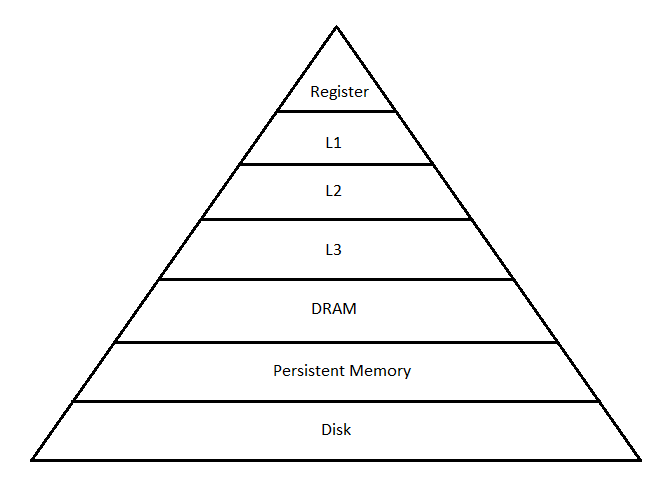
\includegraphics[scale=0.85]{Intro/Pyramid.png}
\caption{Persistent memory becomes a new level between DRAM and Disk\cite{optane}}
\label{fig:Pyramid}
\end{figure}

\subsection{Challenges}

\subsubsection{Security}
One challenge when it comes to persistent memory is security and privacy\cite{Badam}. When an encryption key is used to unlock files, the key is stored in the memory. If it is DRAM then the key will disappear when the computer is shut down, but if it is stored in persistent memory it will persist and remain there until it is deleted. It will be very easy for someone to extract data from persistent memory if the person is able to gain access to it. The same concern also applies to personal information that is being stored in the persistent memory. When developing applications that will use persistent memory and handling sensitive information the programmer needs to remember that data he puts in persistent memory will stay there until it is deleted. It’s also worth mentioning that when the data is deleted or deallocated in the memory, the OS makes the space available to another application. The data is only deleted when its overwritten.

\subsubsection{Durability}
Another challenge for persistent memory is durability. While persistent memory behaves more like DRAM it still has a considerably shorter lifespan than DRAM\cite{Badam}. This is because persistent memory can only write data to a certain amount of time to a region before the region can no longer hold any data reliably. While the storage capacity of persistent memory has increased, so has the bit error rate increased even more. The solution to this is to either have the hardware mask all the regions with bit error from the software or have the hardware expose them to the software and let the software handle the rest. There is also the possibility of letting the hardware and software work together in order to mask regions with bit errors. This will expand the lifespan of persistent memory, but the challenge for hardware producers is to come up with new technologies that can increase the durability of the persistent memory.

\subsubsection{Persistent memory leaks}
A common problem one might have when programming in C concerns memory leaks. When the application is using normal DRAM, the memory consumed by the application can be freed just by restarting the application. If the application is using persistent memory on the other hand, then the memory consumed by the application will remain consumed even after the program has been restarted.\cite{Volos}\cite{Swanson} Memory leaks will persist a shutdown just like persistent memory will. The technology must ensure that the memory occupied on the persistent memory can be tracked down to the application that allocated the memory. By doing this it is possible to track down and remove memory leak for the persistent memory.

\subsection{Advantages}
\subsubsection{Cost}
One of the biggest shortcomings of DRAM is that it is expensive. When the amount of memory increases in a system the cost of DRAM scales nonlinearly.\cite{Badam} This has led to memory becoming a bottleneck in servers that run programs where a lot of memory is needed. Persistent memory is more scalable in terms of cost compared to DRAM. 

This will enable servers to have more storage capacity that can be read at almost the same speed as DRAM.

\subsubsection{Capacity, larger physical memory}
The memory capacity of persistent memory represents a drastic increase in the size of memory that is available to the user. Intel has announced a new persistent memory called Intel Optane DC\cite{side1}. This is a persistent memory that is compatible with a DDR4 socket and each memory module can contain 512 Gigabytes of memory. The bigger memory size will make it possible to keep more of the data the user is working on in the memory and reduce the traffic between the memory and the hard drive.

\subsubsection{Byte addressable, low latency}
Since the persistent memory is connected to a DRAM slot it is also byte-addressable. When a program accesses traditional storage it must wait for the OS to do an I/O block in order to get access which takes a long time and read/write are done in 4 kB blocks. With persistent memory the program can skip the I/O block and access the data directly, this will dramatically decrease the latency. Typical latency when using DRAM would be around 10\textsuperscript{-7} seconds\cite{lerebok} while Intel has measured their Optane DC to have a latency of 4.1 ms\cite{optane2}. Persistent memory is 40 times slower than normal DRAM, but it is still a lot better than SSD that can have 80 ms latency.

\subsection{The rest of thesis}
In Chapter \ref{Chapter:Basicprogramming} there will be an explanation of how to program with NVDIMM. There will be an explanation of some of the different types of libraries that exist. How to set up a memory pool that will be used by the programmer and an explanation of method that will be most used by the programmer. 

In chapter \ref{Chapter:Benchmarks} will be several benchmarks that will show the performance of DRAM and NVDIMM when whey are working alone and when they are working simultaneously. There will also be made observations about the results from the benchmarks.

%There will also be an comparison to see if DRAM and NVDIMM are working faster or slower together when compared to DRAM working alone.

Chapter \ref{Chapter:Cooperation} will be about a scenario that a programmer can encounter. That is when the data exceed the the total capacity of DRAM and the programmer is forced to split the data in two part and place the part that exceeds DRAM on NVDIMM. There will be a formula that calculates how many threads should be reallocated to work on NVDIMM.

Chapter \ref{Chapter:workingIndepandently} will be about a different scenario. The chapter will test the ability of DRAM and NVDIMM to work with two different tasks. The two groups will synchronize by using a lock/unlock function. 

%Chapter five will be about a different scenario. There will be a program with two part. Part one is data is calculated on DRAM by a group of threads. Part two will also have a group of threads that will first transfer the calculated data from DRAM to NVDIMM and analyze the data on NVDIMM. 

Chapter \ref{chapter:conclusion} will contain a summary and a conclusion.

\subsection{Research questions}
This thesis will try to answer the following research questions.
\begin{itemize}
\item What is the data transfer speed of NVDIMM compared to DRAM?
\item In an competitive environment, in what way will NVDIMM and DRAM affect each other?
\item When the size of the data is higher than the capacity of the DRAM, how much data should be transferred to NVDIMM? How many threads should be allocated to work on the data on NVDIMM?
\item While DRAM is working on a task, is it possible for NVDIMM to be working on a different type of task?
\end{itemize}

% - What is the speed of NVDIMM compared to DRAM?\\
% - How does NVDIMM and DRAM interact with each other?\\
% - In an competitive competition how does NVDIMM and DRAM affect each other?
% - How many threads should the user allocate to NVDIMM when data is divided between DRAM and NVDIMM?\\
% - Something about simulation.\\


\clearpage
\section{Basic programming with NVDIMM}
\label{Chapter:Basicprogramming}
% - Creating pmempool
% - Different libraries
% - Opening pool in programm
% - initialzing memory
% - Write memory
% - read memory
\subsection{Introduction}
This chapter will be about how to program with NVDIMM. In order to create code that is using NVDIMM the programmer must choose what library to use and there are many libraries to pick from and all are made for different purposes and have many different types of methods. This chapter exists so others can start on the right track and quickly learn how to use NVDIMM.

The libraries and methods described in this chapter are relevant for NVDIMM devices that support the libraries created by Intel at pmem.io.

\subsection{Different types of libraries}
\subsubsection{Libpmemobj}
Libpmemobj\cite{libpmemobj} allows objects to be stored in persistent memory. The objects in question are not class objects one finds in C++, but instead they are variable-sized blocks of data. The object has an object ID that is independent when it comes to location. The changes or updates to these objects are atomic because the library have transactions to make this happen. This library can be used for multithreading and have been optimized for scaling when it comes to multithreading. The main author also mentions that the C++ version of this library is the cleanest and least prone to error compared to all the other libraries\cite{Rudoff}. He therefore recommends that programmers should start using this library if they are new to persistent memory programming.

\subsubsection{libpmemblk and libpmemlog}
These libraries are made for specific cases. Libpmemblk\cite{libpmemblk} is used for handling large arrays of persistent memory blocks. The blocks must be larger than 512 bytes in order to work. This library is useful if the program is made to manage a block cache. Libpmemlog\cite{libpmemlog} is used to append log files. If the program logs a lot of data, it might be better to use libpmemlog in order to avoid going through the traditional file system where most of the time would be spent waiting.

\subsection{Creating pmempool}
\label{section:memorypool}
%pmempool create --layout my_layout --size=50G obj pool.obj
Before NVDIMM can be used, the user must create what is called a memory pool on the NVDIMM. The NVDIMM has several modes, in order to be able to create a memory pool the mode must be set to fsdax. On a server this must be done by the system administrator. To see what mode the NVDIMM is in can be done by the command ndctl-list. A program called pmempool must also be installed on the server, it is this program that will create the memory pool.
The command used for creating the memory pool for this thesis is 
\begin{lstlisting}
pmempool create --layout Layout_name --size=170G obj pool.obj
\end{lstlisting}
The layout is a string stored in the memory pool. When a program accesses a memory pool it needs to send a string that matches the string in the memory pool in order to use it. The user can specify the size of the memory pool, if size is not specified the pmempool will create a pool with the lowest size allowed.
There are three different types of memory pool to choose from, they are obj, log and blk. Which type of memory pool to use depends on which type of library is used in the program. In this thesis the libpmemobj library was used and that is why obj was used in the creating of memory pool. Log and blk are for the libraries libpmemlog and libpmemblk.
The last part of the command line is the name and file address of the memory pool.

\subsection{NVDIMM Functions used in thesis}
In this project it is the libpmemobj library that will be used. Below is a short description of all the functions that will be used in the thesis. 
\subsubsection{Open memory pool}
\label{subsection:openmemorypool}
The memory pool uses a pointer called PMEMobjpool. The memory pool is opened by using the method pmemobj\_open that needs two arguments. The first argument is the path to the memory pool created in chapter \ref{section:memorypool}. The second argument is a text string that identifies what data belongs to what program.
\begin{lstlisting}
PMEMobjpool *pop = pmemobj_open(path, LAYOUT_NAME);
\end{lstlisting}

\subsubsection{Declaring an array}
When the programmer wants to declare an array, the follow command must be used.
\begin{lstlisting}
TOID(Type) Array_name;
\end{lstlisting}
Type is the data type the programmer wants to use and the name is the name of the array.

\subsubsection{Allocating array}
When allocating the array the method called POBJ\_ALLOC is used. The method has six arguments. The first argument is the memory pool created in chapter \ref{subsection:openmemorypool}. The second argument is the the array the user wants to allocate memory. Third argument is the data type and the fourth argument is the array length in bytes. The last two arguments are irrelevant in this context and can be given the value NULL.\\
\begin{lstlisting}
//Allocating of the array
POBJ_ALLOC(Memory_pool, &Array_name, Type, sizeof(double) * ARRAY_LENGTH, NULL, NULL);
//Deallocating of the array
POBJ_FREE(&Array_name);
\end{lstlisting}
When the user want to deallocate the array the function POBJ\_FREE must be used. The function is similar to the free function when using malloc. The user only need to the name of the they want to deallocate as argument in POBJ\_FREE. 
%When deallocating the array the method POBJ\_FREE that only need the array the user want to deallocate as argument.

\subsubsection{Read/Write to array}
%When reading and writing to an array, the following command are used
This section will explain the function D\_RO and D\_RW which stands for DIRECT\_RO and DIRECT\_RW and they will read and write directly to the NVDIMM array.
Reading from the array is done by using the method D\_RO that must have the array the user wants to read from as argument. The method also uses square brackets after the argument that needs the index of the element in the array the user want to read. The method D\_RW is used when reading to the array. The use of this method is identical to D\_RO.
\begin{lstlisting}
//Reading an array variable.
var = D_RO(Array_name)[index];

//Writing to an array variable.
D_RW(Array_name)[index] = var;
\end{lstlisting}



\subsection{Coding example}
This is an example on how to use the pmemobj library. The example will find the average of an array where the array is replaced with an NVDIMM array. The purpose is to show how easy it is to code with NVDIMM by having all the relevant methods in an easy example.
The way of using the a NVDIMM library is a lot similar to using ordinary arrays. Once the programmer has chosen what NVDIMM library to use and included the library in the code the memory pool must be opened. The first thing the code needs is the path to the memory pool and a layout, which is a string that identifies the pool that the user can choose what it will be. This can either be a command line argument the user gives when starting the program or it can be hard coded into the code. This is what has been done in listing \ref{nvdimm_example} at line 5 and 11. These two strings are used as arguments when initiating the pool at line 14-15. The initiation is also followed up with an if-sentence at line 16-19 to check that the memory pool has been successfully created. If it has not the program will print out an error message and exit the program.

Next is to create a NVDIMM array, this is what happens at line 21. The NVDIMM array pointer is a void pointer that is casted to a double pointer. 
The array gets initiated at line 22. The method used is called POBJ\_ALLOC, this method is similar to malloc for DRAM. The method has six arguments, the first argument is what memory pool the array will be assigned to.
The second argument is the address of the pointer. Third argument is the type of the elements in the array. The fourth argument is the length of the array, that is the size of type multiplied with the number of elements in array. The last two arguments are set to NULL.

When writing to an NVDIMM array the programmer must use the method called D\_RW. It only has one argument which is the name of the array. It is followed up with a pair square brackets that contains the index of the element the programmer wants to write to, an example can be found at line 25.

D\_RO is the name of the method one must use to read an element from an NVDIMM array. This method also has one argument which is the name of the array and the square brackets contains the index of the element that will be read. Line 29 is an example of how to add the value of an element in a NVDIMM array to a variable.

In order to deallocate the a NVDIMM array one must use the method POBJ\_FREE and the only argument needed is the address of the \\NVDIMM pointer, an example can be found in line 34. If the programmer forgets to free up the NVDIMM array there will be a permanent memory leak that will last even after the program have stopped running. In order to get rid of the memory leak one must delete the memory pool and create a new one.

Lastly one must close the memory pool before the program is terminated. This is done with pmemobj\_close, it only has the pointer for the memory pool as argument. Line 35 shows how to close the memory pool.

The functions introduced in this chapter will be used in all the other chapters where I create new benchmarks and tests.

%POBJ_ALLOC(PMEMobjpool *pop, TOID *oidp, TYPE, size_t size, pmemobj_constr constructor, void *arg)
\begin{lstlisting}[caption={Example of coding with NVDIMM}, label={nvdimm_example}]
#include <stdio.h>
#include <stdlib.h>
#include <libpmemobj.h>

POBJ_LAYOUT_BEGIN(array);
POBJ_LAYOUT_TOID(array, double);
POBJ_LAYOUT_END(array);

#define ARRAY_LENGTH 1000
#define LAYOUT_NAME "my_layout"
int main(int argc, char *argv[])
{
	double average = 0.0;
	int i;
	//The path for the memory pool.
	const char path[] = "/mnt/pmem1-ext4/pool.obj";
	
	/* create the pmemobj pool or open it if it already exists */
	PMEMobjpool *pop;
	pop = pmemobj_open(path, LAYOUT_NAME);
	if (pop == NULL) {
		perror(path);
		exit(1);
	}
	//Creation of NVDIMM array.
	TOID(double) nvm_array;
	POBJ_ALLOC(pop, &nvm_array, double, sizeof(double) * ARRAY_LENGTH, NULL, NULL);
	//Writing to the array.
	for(i=0;i<ARRAY_LENGTH;i++){
		D_RW(nvm_array)[i] = i;
	}
	//Reading from the NVDIMM array.
	for(i=0;i<ARRAY_LENGTH;i++){
		average += D_RO(nvm_array)[i];
	}
	average = average / ARRAY_LENGTH;
	printf("%f\n", average);
	
	POBJ_FREE(&nvm_array);
	pmemobj_close(pop);
	return 0;
}
\end{lstlisting}


\clearpage
\section{Benchmarks}
\label{Chapter:Benchmarks}
%There are four different benchmarks.
\subsection{Introduction}
Persistence memory is slower than DRAM. But there is not much information on how much slower the NVDIMM is in comparison to DRAM. This chapter will test the performance of NVDIMM when it work alone and when it works simultaneously with DRAM. The results will be presented with graphs and tables that will show the difference in performance.
The chapter will start off with using the STREAM\cite{STREAM-c} benchmark in order to find the performance of DRAM.
The NVDIMM will also be tested with a STREAM benchmark that have been modified by me for this thesis. 
Three original benchmarks will also test the NVDIMM when it works simultaneously with DRAM.
In the first benchmark DRAM will copy an array from DRAM while NVDIMM copies an array from NVDIMM. 
In the second benchmark DRAM will copy from DRAM while NVDIMM will copy an array to DRAM. In the last benchmark DRAM will copy from DRAM while NVDIMM will copy an array from DRAM.

\subsubsection{Hardware}
\label{sec:hardware}
All the benchmarks has been tested on a server with the following hardware.\\
Motherboard: Supermicro X11DPU-Z+ \\
CPU: Intel(R) Xeon(R) Gold 6130 CPU @ 2.10GHz, 16 cores \\
DRAM: Samsung RDIMM, 2666 MT/s. \\
NVDIMM: Micron Technology NV-DIMM , 2933 MT/s \\
\\
The server have two CPU, both CPU have twelve memory slots each. Each CPU have six channels. There are one DRAM and one NVDIMM sharing one channel.
The compiler used to compile the code is gcc (Ubuntu 7.5.0-3ubuntu1~18.04) 7.5.0. The code have been optimized to level two (-o2).

All of the benchmarks have been tested on socket two. This is to avoid disturbances as much as possible since most of the other processes are running on socket one.

\subsection{STREAM DRAM}
\label{section:STREAMDRAM}
The STREAM\cite{STREAM-c} benchmark is a synthetic and simple benchmark that is designed to measure bandwidth in MB/s. This benchmark is seen as the standard for measuring memory bandwidth and has not been modified in any way after it was downloaded from the creator websites.
The benchmark tests memory bandwidth by running four different tests. The first one test is copy where the elements in one array are copied to another array.
The second test is called scale where each element is multiplied with a constant and the result is placed in a second array, the index of the element in the first array and the result in the second array is the same.
Third test is add where the elements from two different arrays with the same index are added together and place in a third array where the index is the same as in the two other arrays.
Last test is the triad where the one array is multiplied with a constant then added together with a second array and then placed in a third array.

The DRAM Stream benchmark runs the test 32 times and only on one socket, every time it restarts with one extra thread is added. The CPU has 16 cores and when the thread number surpasses that number it starts using the hyper threads on the same core. The Linux program numactl is also used to manage the number of threads and what socket the benchmark is allowed to use.

The result shown in figure \ref{fig:DRAM_STREAM_100M_Figure} and table \ref{tab:DRAM_STREAM_100M_Table} is what was expected, adding more threads in beginning will give a big increase in transfer speed. But at thread 5 the gains in transfer speed will start to diminish and at thread 11 there will be very little increase in transfer speed when adding more threads.
This means that it might be possible to allocate five of the sixteen threads to work on NVDIMM and not loose a significant amount of performance for the eleven remaining threads that are still working on DRAM. 

After sixteen threads the benchmark starts to use the hyper-threads. There is a 10,000 MB/s decrease when the benchmark starts to use the hyper-threads. When more and more hyper-threads are added the bandwidth will increase until it is almost at the same level when there were only sixteen threads. 32 threads have 2,000 MB/s lower bandwidth than sixteen threads.

\begin{figure}[!hbtp]
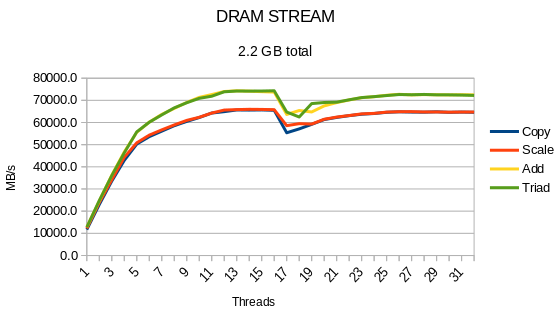
\includegraphics[scale=0.7]{Benchmarks/DRAM_STREAM_100M_Figure.png}
\caption{DRAM Stream, 2.2 GB total. Graph of table \ref{tab:DRAM_STREAM_100M_Table}.}
\label{fig:DRAM_STREAM_100M_Figure}
\end{figure}

\begin{table}[!hbtp]
\centering
\begin{tabular}{ |c|c|c|c|c| }
\hline
Threads & Copy & Scale & Add & Triad \\
\hline
1 & 11673.5 & 12180.6 & 12799.4 & 12745.3 \\
\hline
2 & 22995.1 & 23892.4 & 24637.1 & 24807.8 \\
\hline
3 & 33554.9 & 34206.9 & 36248.9 & 36070.7 \\
\hline
4 & 42917.3 & 44315.0 & 46759.0 & 46333.7 \\
\hline
5 & 50260.9 & 50853.1 & 55574.9 & 55784.3 \\
\hline
6 & 53612.5 & 54305.3 & 60174.4 & 60129.4 \\
\hline
7 & 56100.8 & 56671.2 & 63670.6 & 63425.1 \\
\hline
8 & 58554.6 & 58888.6 & 66348.1 & 66607.5 \\
\hline
9 & 60491.7 & 60947.7 & 69059.1 & 68923.9 \\
\hline
10 & 62242.2 & 62368.3 & 71335.2 & 70900.6 \\
\hline
11 & 64257.1 & 64270.1 & 72604.0 & 71854.1 \\
\hline
12 & 64890.3 & 65611.6 & 73973.6 & 73866.7 \\
\hline
13 & 65648.8 & 65805.9 & 74285.3 & 74204.8 \\
\hline
14 & 65606.5 & 65943.6 & 74128.9 & 74158.9 \\
\hline
15 & 65665.5 & 65897.7 & 73918.8 & 74199.9 \\
\hline
16 & 65509.8 & 65770.4 & 73721.2 & 74312.2 \\
\hline
17 & 55365.3 & 58578.1 & 63624.8 & 64728.6 \\
\hline
18 & 57104.2 & 59481.5 & 65404.0 & 62472.2 \\
\hline
19 & 59160.6 & 59279.3 & 64749.4 & 68522.2 \\
\hline
20 & 61328.6 & 61453.3 & 67489.5 & 69020.7 \\
\hline
21 & 62290.7 & 62453.6 & 68987.6 & 69178.2 \\
\hline
22 & 63091.2 & 63146.4 & 70173.6 & 70239.2 \\
\hline
23 & 63737.2 & 63887.6 & 71195.5 & 71235.8 \\
\hline
24 & 64056.6 & 64108.0 & 71629.1 & 71669.4 \\
\hline
25 & 64601.7 & 64685.7 & 72282.9 & 72167.3 \\
\hline
26 & 64824.5 & 64850.8 & 72729.4 & 72623.9 \\
\hline
27 & 64706.3 & 64890.3 & 72444.1 & 72525.6 \\
\hline
28 & 64654.6 & 64743.1 & 72586.7 & 72656.9 \\
\hline
29 & 64827.0 & 64750.6 & 72505.7 & 72481.2 \\
\hline
30 & 64589.2 & 64659.6 & 72453.0 & 72472.8 \\
\hline
31 & 64703.8 & 64714.4 & 72531.8 & 72356.7 \\
\hline
32 & 64610.4 & 64721.9 & 72459.3 & 72212.9 \\
\hline
\end{tabular}
\caption{DRAM Stream, 2.2 GB total. Speed are in MB/s.}
\label{tab:DRAM_STREAM_100M_Table}
\end{table}

%\clearpage
\subsection{STREAM NVDIMM}
\label{section:STREAM_NVDIMM}
The stream NVDIMM benchmark measures the memory speed of the NVDIMM. This benchmark is the same as the STREAM benchmark has been described in chapter \ref{section:STREAMDRAM}. The difference is that the memory type has been changed from DRAM to NVDIMM by me.
The code shown in listing \ref{lst:orgStreamDram} is part of the original code that has been removed from the code.
\begin{lstlisting}[caption={Original STREAM benchmark code at line 175-181.}, label={lst:orgStreamDram}]
#ifndef STREAM_TYPE
#define STREAM_TYPE double
#endif

static STREAM_TYPE  a[STREAM_ARRAY_SIZE+OFFSET],
                    b[STREAM_ARRAY_SIZE+OFFSET],
                    c[STREAM_ARRAY_SIZE+OFFSET];
\end{lstlisting}
It has been replaced with the code shown in listing \ref{lst:orgStreamNvdimm}. The code starts by opening the memory pool at line 21-27. The code will use a method called initiate at line 28 that will initiate the three arrays. Once this is done the code will continue executing the rest of the STREAM benchmark code just like the original code. The difference is that lines with read or write to DRAM array has been replaced with the functions D\_RO and D\_RW which read and write to NVDIMM.
\begin{lstlisting}[caption={Code that has replaced original code.}, label={lst:orgStreamNvdimm}]
PMEMobjpool *pop;
POBJ_LAYOUT_BEGIN(array);
POBJ_LAYOUT_TOID(array, double);
POBJ_LAYOUT_END(array);
//Declearing the arrays
TOID(double) a;
TOID(double) b;
TOID(double) c;

void initiate()
{
	//Initiating the arrays.
	POBJ_ALLOC(pop, &a, double, (STREAM_ARRAY_SIZE+OFFSET)*sizeof(STREAM_TYPE), NULL, NULL);
	POBJ_ALLOC(pop, &b, double, (STREAM_ARRAY_SIZE+OFFSET)*sizeof(STREAM_TYPE), NULL, NULL);
	POBJ_ALLOC(pop, &c, double, (STREAM_ARRAY_SIZE+OFFSET)*sizeof(STREAM_TYPE), NULL, NULL);
}

int main()
{
	const char path[] = "/mnt/pmem1-ext4/pool.obj";
	pop = pmemobj_create(path, LAYOUT_NAME, 10737418240, 0666);
	if (pop == NULL)
		pop = pmemobj_open(path, LAYOUT_NAME);
	if (pop == NULL) {
		perror(path);
		exit(1);
	}
	initiate();
	//The rest of the STREAM benchmark after this.
}
\end{lstlisting}

The result on the NVDIMM Stream benchmark shown in figure \ref{fig:NVM_STREAM_100M_Figure} and table \ref{tab:NVM_STREAM_100M_Table} is very different from the DRAM Stream benchmark. The DRAM Stream benchmark had a steep increase in bandwidth in the beginning that started to taper off at thread five and almost no increase from thread eleven. The NVDIMM has a more linear increase in bandwidth when the threads are increased from one thread towards sixteen threads. 
This might be because the speed of one thread is half the bandwidth of one thread in the DRAM Stream benchmark. 
The max bandwidth reached by the NVDIMM Stream benchmark is 51,273 MB/s and the DRAM Stream benchmark starts to taper off at around 55,000 MB/s. The NVDIMM Stream benchmark never reaches a speed high enough so it can start to taper off and therefore it look more like linear increase in bandwidth.

Thread seventeen and after are the hyper-threads and at thread seventeen there is a 15,000 MB/s decrease before the bandwidth overall start to increase with more hyper-threads added. The bandwidth swings up and down a lot. There is no clear explanation on why the bandwidth fluctuates so much. 

\begin{figure}[!hbtp]
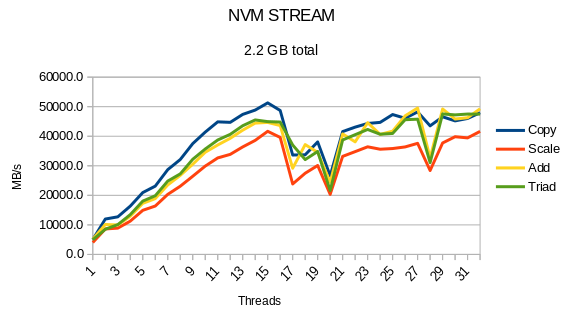
\includegraphics[scale=0.7]{Benchmarks/NVM_STREAM_100M_Figure.png}
\caption{NVDIMM Stream, 2.2 GB total. Graph of table \ref{tab:NVM_STREAM_100M_Table}.}
\label{fig:NVM_STREAM_100M_Figure}
\end{figure}

\begin{table}[!hbtp]
\centering
\begin{tabular}{ |c|c|c|c|c| } 
\hline
Threads & Copy & Scale & Add & Triad \\
\hline
1 & 5036.7 & 4026.4 & 5151.3 & 4956.0 \\
\hline
2 & 11970.2 & 8616.8 & 10120.7 & 8515.8 \\
\hline
3 & 12715.1 & 8903.4 & 9972.6 & 10085.0 \\
\hline
4 & 16349.6 & 11266.2 & 12922.7 & 13474.2 \\
\hline
5 & 20935.0 & 14924.3 & 17282.1 & 18050.7 \\
\hline
6 & 23119.7 & 16381.2 & 18887.2 & 19859.8 \\
\hline
7 & 28694.5 & 20320.0 & 23509.8 & 24824.9 \\
\hline
8 & 32104.6 & 23082.0 & 26744.5 & 27255.4 \\
\hline
9 & 37491.8 & 26450.3 & 30517.3 & 32194.4 \\
\hline
10 & 41394.8 & 29897.7 & 34575.6 & 35671.3 \\
\hline
11 & 44856.8 & 32659.1 & 37032.5 & 38714.6 \\
\hline
12 & 44695.1 & 33848.9 & 39292.6 & 40625.8 \\
\hline
13 & 47377.9 & 36377.7 & 42050.6 & 43542.1 \\
\hline
14 & 48853.3 & 38589.6 & 44440.4 & 45509.7 \\
\hline
15 & 51273.9 & 41662.3 & 44663.6 & 44941.4 \\
\hline
16 & 48704.8 & 39592.3 & 43615.7 & 44797.8 \\
\hline
17 & 33638.9 & 23842.9 & 29161.2 & 37024.5 \\
\hline
18 & 33712.5 & 27466.9 & 37166.7 & 32095.5 \\
\hline
19 & 38073.6 & 30095.0 & 34539.9 & 34835.6 \\
\hline
20 & 26627.1 & 20307.7 & 24445.4 & 21617.2 \\
\hline
21 & 41575.9 & 33180.5 & 40777.5 & 38727.8 \\
\hline
22 & 43078.1 & 34787.1 & 38100.6 & 40516.5 \\
\hline
23 & 44306.5 & 36409.9 & 44583.9 & 42289.1 \\
\hline
24 & 44679.1 & 35595.9 & 40602.3 & 40671.9 \\
\hline
25 & 47327.4 & 35824.6 & 41718.8 & 40939.5 \\
\hline
26 & 46085.6 & 36378.7 & 46893.2 & 45583.9 \\
\hline
27 & 48237.8 & 37579.8 & 49538.8 & 45762.3 \\
\hline
28 & 43507.7 & 28391.9 & 32673.6 & 31051.1 \\
\hline
29 & 46562.0 & 37710.1 & 49211.6 & 47533.4 \\
\hline
30 & 45188.7 & 39833.6 & 45820.8 & 47210.6 \\
\hline
31 & 46011.6 & 39429.2 & 46247.3 & 47491.9 \\
\hline
32 & 47961.6 & 41638.6 & 49278.3 & 47481.3 \\
\hline
\end{tabular}
\caption{NVDIMM Stream, 2.2 GB total. Speeds are in MB/s}
\label{tab:NVM_STREAM_100M_Table}
\end{table}

%\clearpage
\pagebreak
\subsection{Competition benchmarks}
This section is about three new benchmarks. In the first benchmark data will be copied from a DRAM array to another DRAM array and from a NVDIMM array to another NVDIMM array simultaneously. In the second benchmark data will be copied from a DRAM array to another DRAM arrays and from a DRAM array to a NVDIMM array simultaneously. In the last benchmark data will be copied from a DRAM array to another DRAM array and from a NVDIMM array to a DRAM array simultaneously.

The purpose of these benchmarks is to get an understanding of how performance will be affected when different threads generate traffic from DRAM and NVDIMM simultaneously. That is why there are three types of benchmarks in order to test all possible combination of traffic. 

\subsubsection{NVM-NVM}
\label{section:NVM-NVM}
The code for this benchmark is described in listing \ref{lst:NVMNVMcode}.
From line 2-14 the code is declaring variables and creating the arrays where the result from the benchmark will be stored. There will be declared two DRAM arrays and two NVDIMM arrays that will be used in the benchmark.
When the threads arrive at line 16 they will synchronize before they are split into two groups. Threads with a thread id lower than the number of DRAM threads will pass the if-sentence at line 17, where they will initiate two DRAM arrays and place values into each element.
The rest of the threads will move on to line 27 and enter this bracket. These threads will initiate two NVDIMM arrays and place values into each element.
All the threads will then synchronize at line 40 before they will divide into two groups at line 41 in the same fashion they did in line 17. All the threads will then start to copy data from one array to the other array. The DRAM threads will copy one of the DRAM array to the other DRAM array and the NVDIMM threads will copy one of the NVDIMM array to the other NVDIMM array. They will repeat this for as many times as the user of the benchmark has decided by defining the total\_test variable as an argument in the command line when the program was started. The time measurement will be started at the beginning of the for-loop at line 45 or 54 and end at the end of the for-loop at line 50 or 60.
When the benchmark testing is over the threads will free up their arrays and the benchmark will print out the result. 

When the threads pass the barrier at line 40 and begin the benchmark test they will never synchronize another time. Because of this the DRAM threads will complete their tasks earlier than NVDIMM threads because DRAM speed is faster then NVIDMM speed. This also means that once the fastest thread is done the rest of the threads will share more bandwidth among  them self and become faster. When more and more threads complete their tasks the faster the remaining threads will become.
In order to get a correct benchmark where all threads have been working the user must not use  data where some threads are working when other threads have completed their tasks. Throwing out the last one third of the raw data is usually enough.
There is also a need to throw out at least the first 25 iterations. This is because the NVDIMM is a lot slower to get started than DRAM. 

\begin{lstlisting}[caption={NVM-NVM source code.},escapeinside={{/*!}{!*/}}, label={lst:NVMNVMcode}]
#pragma omp parallel
{
	//Declearing variables.
	int thread_id = omp_get_thread_num();
	int i,j;
	double *drm_read_array;
	double *drm_write_array;
	TOID(double) nvm_read_array;
	TOID(double) nvm_write_array;
	srand((unsigned int)time(NULL));	
	#pragma omp master
	{
		/* Creates array where the test result will be added. */
	}	
	//Creates all the arrays needed for the test.
	#pragma omp barrier
	if(thread_id < totalThreads-nvmThreads){
		drm_read_array = (double*)malloc(ARRAY_LENGTH*sizeof(double));
        drm_write_array = (double*)malloc(ARRAY_LENGTH*sizeof(double));
		#pragma omp critical
		{
			for(i=0;i<ARRAY_LENGTH;i++){
				drm_read_array[i] = ((double)rand()/(double)(RAND_MAX));
				drm_write_array[i] = ((double)rand()/(double)(RAND_MAX));
			}
		}
	}else if(thread_id >= totalThreads-nvmThreads){
		POBJ_ALLOC(pop, &nvm_read_array, double, sizeof(double) * ARRAY_LENGTH, NULL, NULL);
		POBJ_ALLOC(pop, &nvm_write_array, double, sizeof(double) * ARRAY_LENGTH, NULL, NULL);
		#pragma omp critical
		{
			for(i=0;i<ARRAY_LENGTH;i++){
				D_RW(nvm_read_array)[i] = ((double)rand()/(double)(RAND_MAX));
				D_RW(nvm_write_array)[i] = ((double)rand()/(double)(RAND_MAX));
			}
			//printf("NVM thread_id: %d, %f\n", thread_id, D_RO(nvm_read_array)[11235]);
		}
	}
	//Doing the test.
	#pragma omp barrier
	if(thread_id < totalThreads-nvmThreads){
		//From DRAM to DRAM:
		for(i=0;i<total_tests;i++){
			//Time start
			test_time[thread_id][i] = mysecond();
			for(j=0;j<ARRAY_LENGTH;j++){
				drm_write_array[j] = drm_read_array[j];
			}
			//Time stop.
			test_time[thread_id][i] = mysecond() - test_time[thread_id][i];
		}
	}else if(thread_id >= totalThreads-nvmThreads){
		//From NVM to NVM:
		for(i=0;i<total_tests;i++){
			//Time start
			test_time[thread_id][i] = mysecond2();
			for(j=0;j<ARRAY_LENGTH;j++)
				D_RW(nvm_write_array)[j] = D_RO(nvm_read_array)[j];
			//Time stop.
			test_time[thread_id][i] = mysecond2() - test_time[thread_id][i];
		}
	}else
		printf("ERROR\n");
	/* Freeing up DRAM and NVDIMM arrays */
}
\end{lstlisting}

%\clearpage
\begin{table}[!hbtp]
\centering
\begin{tabular}{ |c|c|c|c|c| } 
\hline
DRAM & NVDIMM &  & & \\
threads & threads & DRAM & NVDIMM & Sum \\
\hline
15 & 1 & 61042.84 & 3038.16 & 64081.01 \\
\hline
14 & 2 & 57761.80 & 6027.24 & 63789.03 \\
\hline
13 & 3 & 53767.10 & 9223.43 & 62990.52 \\
\hline
12 & 4 & 51257.79 & 12630.42 & 63888.22 \\
\hline
11 & 5 & 47770.89 & 15202.48 & 62973.37 \\
\hline
10 & 6 & 43771.07 & 18771.08 & 62542.15 \\
\hline
9 & 7 & 39780.16 & 22085.75 & 61865.90 \\
\hline
8 & 8 & 36275.70 & 25068.35 & 61344.05 \\
\hline
7 & 9 & 31873.99 & 28520.43 & 60394.42 \\
\hline
6 & 10 & 28691.82 & 30840.40 & 59532.22 \\
\hline
5 & 11 & 24580.59 & 33991.75 & 58572.33 \\
\hline
4 & 12 & 20550.17 & 38006.44 & 58556.61 \\
\hline
3 & 13 & 15877.24 & 40011.90 & 55889.14 \\
\hline
2 & 14 & 11010.71 & 43913.44 & 54924.15 \\
\hline
1 & 15 & 5932.95 & 46352.16 & 52285.11 \\
\hline
\end{tabular}
\caption{NVM-NVM, 32 GB total. DRAM and NVDIMM threads competing for bandwidth. Speeds are in MB/s.}
\label{tab:NVM_NVM}
\end{table}

The result of the benchmark is shown in figure \ref{fig:NVM_NVM} and table \ref{tab:NVM_NVM}. They show that as the number of NVDIMM threads increases at the expense of the DRAM threads the NVDIMM bandwidth increases and DRAM bandwidth decreases. 
The sum of the DRAM and NVDIMM starts at 64,081 MB/s and decreases with 1,100 MB/s when there are five NVDIMM threads. When the number of NVDIMM threads increases even more, the bandwidth decreases at a  higher rate. From five to fifteen NVDIMM threads the bandwidth has decreased with 10,000 MB/s. This might be because the NVDIMM is not fast enough to make use of all the bandwidth that becomes available as the number of DRAM threads decreases. The result is that the user loses performance if the number of NVDIMM is too high.

\begin{figure}[!hbtp]
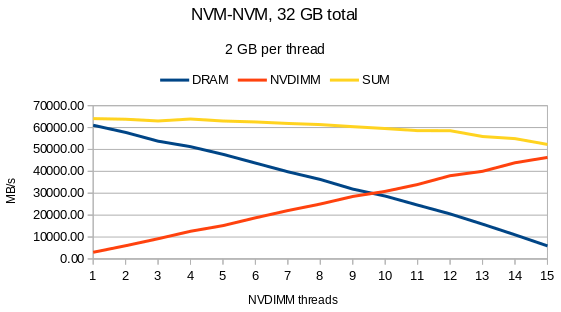
\includegraphics[scale=0.7]{Benchmarks/NVM-NVM_32GB_Figure.png}
\caption{Graph of table \ref{tab:NVM_NVM}. DRAM and NVDIMM threads competing for bandwidth.}
\label{fig:NVM_NVM}
\end{figure}

%\clearpage
%New graphs with second on x-axis and bandwidth on Y-axis. 500 iterations.
The graph in figure \ref{fig:NVM_NVM_sec} is the result of the same benchmark as figure \ref{fig:NVM_NVM}. The difference is that figure \ref{fig:NVM_NVM_sec} now shows the number of seconds on x-axis and bandwidth on y-axis. Threads ends at different times. The last DRAM ends at 231 seconds and the last NVDIMM ends at around 319 seconds. The figure \ref{fig:NVM_NVM_sec} also shows that all the DRAM threads have the same consistent speed except for the end of the DRAM. The NVDIMM threads on the other hand fluctuate a lot, they seem to have a speed at around 3,000 MB/s, but once in a while they drop down to 1,700 MB/s.
%[!hbtp]
\begin{figure}[btp]
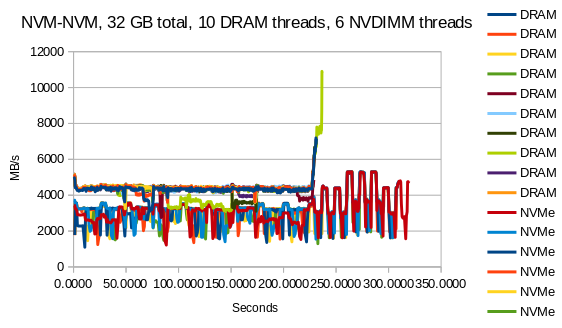
\includegraphics[scale=0.7]{Benchmarks/NVM-NVM_32GB_6_Thread.png}
\caption{DRAM and NVDIMM threads competing for bandwidth over a certain time period. Threads ends at different times.}
\label{fig:NVM_NVM_sec}
\end{figure}

%\clearpage
\pagebreak
\subsubsection{NVM-DRAM}
\label{section:NVM-DRAM}
In this version of the benchmark there will be one group of threads that will transfer data from a DRAM array to a DRAM array and another group of threads that will transfer data from a NVDIMM array to a DRAM array. This code is very similar to the previous code. The differences are at line 26-36 where the code will initiate and add values to one DRAM array and one NVDIMM array instead of two NVDIMM arrays.  
The other difference is at line 51-61 where the code will copy data from NVDIMM-DRAM instead of NVDIMM-NVDIMM. 

\begin{lstlisting}[caption={NVM-DRAM source code.},escapeinside={{/*!}{!*/}}]
#pragma omp parallel
{
	int thread_id = omp_get_thread_num();
	int i,j;
	double *drm_read_array;
	double *drm_write_array;
	TOID(double) nvm_read_array;
	srand((unsigned int)time(NULL));	
	#pragma omp master
	{
		/* Creates array where the test result will be added. */
	}
	//Creates all the arrays needed for the test.
	#pragma omp barrier
	if(thread_id < totalThreads-nvmThreads){
		drm_read_array = (double*)malloc(ARRAY_LENGTH*sizeof(double));
		drm_write_array = (double*)malloc(ARRAY_LENGTH*sizeof(double));
		#pragma omp critical
		{
			for(i=0;i<ARRAY_LENGTH;i++){
				drm_read_array[i] = ((double)rand()/(double)(RAND_MAX));
				drm_write_array[i] = ((double)rand()/(double)(RAND_MAX));
			}
		}
	}
	else if(thread_id >= totalThreads-nvmThreads){
		drm_write_array = (double*)malloc(ARRAY_LENGTH*sizeof(double));
		POBJ_ALLOC(pop, &nvm_read_array, double, sizeof(double) * ARRAY_LENGTH, NULL, NULL);
		#pragma omp critical
		{
			for(i=0;i<ARRAY_LENGTH;i++){
				D_RW(nvm_read_array)[i] = ((double)rand()/(double)(RAND_MAX));
				drm_write_array[i] = ((double)rand()/(double)(RAND_MAX));
			}
		}
	}
	//Doing the test.
	#pragma omp barrier
	if(thread_id < totalThreads-nvmThreads){
		//From DRAM to DRAM:
		for(i=0;i<total_tests;i++){
			//Time start
			test_time[thread_id][i] = mysecond();
			for(j=0;j<ARRAY_LENGTH;j++){
				drm_write_array[j] = drm_read_array[j];
			}
			//Time stop.
			test_time[thread_id][i] = mysecond() - test_time[thread_id][i];
		}
	}
	else if(thread_id >= totalThreads-nvmThreads){
		//From NVM to DRAM:
		for(i=0;i<total_tests;i++){
			//Time start
			test_time[thread_id][i] = mysecond();
			for(j=0;j<ARRAY_LENGTH;j++)
				drm_write_array[j] = D_RO(nvm_read_array)[j];
			//Time stop.
			test_time[thread_id][i] = mysecond() - test_time[thread_id][i];
		}
	}
	else
		printf("ERROR\n");
	/* Freeing up DRAM and NVDIMM arrays */
}
\end{lstlisting}

\begin{table}[!hbtp]
\centering
\begin{tabular}{ |c|c|c|c|c| } 
\hline
DRAM & NVDIMM & & & \\
threads & threads & DRAM & NVDIMM & Sum \\
\hline
15 & 1 & 61257.14 & 3742.24 & 64999.37 \\
\hline
14 & 2 & 58419.89 & 6691.30 & 65111.18 \\
\hline
13 & 3 & 54544.07 & 10520.34 & 65064.41 \\
\hline
12 & 4 & 49997.69 & 15247.47 & 65245.16 \\
\hline
11 & 5 & 46226.88 & 19189.81 & 65416.69 \\
\hline
10 & 6 & 42942.39 & 22806.13 & 65748.52 \\
\hline
9 & 7 & 38156.47 & 27257.45 & 65413.92 \\
\hline
8 & 8 & 34613.22 & 30474.15 & 65087.37 \\
\hline
7 & 9 & 30458.70 & 34533.35 & 64992.05 \\
\hline
6 & 10 & 25489.86 & 39324.61 & 64814.47 \\
\hline
5 & 11 & 22083.85 & 42763.51 & 64847.36 \\
\hline
4 & 12 & 17704.90 & 47147.70 & 64852.60 \\
\hline
3 & 13 & 13394.67 & 51380.63 & 64775.31 \\
\hline
2 & 14 & 8947.75 & 56009.92 & 64957.67 \\
\hline
1 & 15 & 4489.12 & 60031.12 & 64520.24 \\
\hline
\end{tabular}
\caption{NVM-DRAM, 32 GB total. DRAM and NVDIMM threads competing for bandwidth. Speed are in MB/s.}
\label{tab:NVM_DRAM}
\end{table}

The result of this benchmark are shown in figure \ref{fig:NVM_DRAM} and table \ref{tab:NVM_DRAM}. Figure \ref{fig:NVM_DRAM} show that when the number of NVDIMM threads increases the NVDIMM bandwidth also goes up while the DRAM threads and bandwidth goes down. The sum of the DRAM and NVDIMM bandwidth is stable at around 64,000 MB/s for all numbers of NVDIMM threads. 

\begin{figure}[!hbtp]
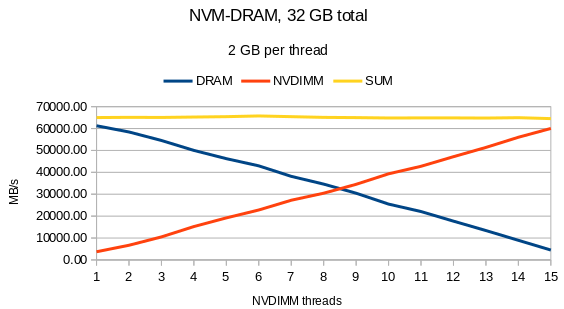
\includegraphics[scale=0.7]{Benchmarks/NVM-DRAM_32GB_Figure.png}
\caption{Graph of table \ref{tab:NVM_DRAM}. DRAM and NVDIMM threads competing for bandwidth.}
\label{fig:NVM_DRAM}
\end{figure}
\pagebreak
Figure \ref{fig:NVM_DRAM_sec1} and \ref{fig:NVM_DRAM_sec2} shows the result of the same benchmark as figure \ref{fig:NVM_DRAM}, but with second on the x-axis instead of NVDIMM threads. Figure  \ref{fig:NVM_DRAM} has been split in two in order to make it more readable, figure \ref{fig:NVM_DRAM_sec1} shows all the DRAM and figure \ref{fig:NVM_DRAM_sec2} shows all the NVDIMM threads.
The last DRAM thread ends at 234 seconds and the last NVDIMM thread ends at 258 seconds. The DRAM threads have consistent speed through the entire test at around 4,300 MB/s, only at the end will the speed increase because other threads have finished before them and therefore made more bandwidth available for the remaining threads. The NVDIMM threads are also more consistent in this benchmark where five of the six threads have speed of 3,800 MB/s for most of the test. There is only one thread that is fluctuating between 3,000 MB/s and 3,600 MB/s for most of the benchmark.

%Figure \ref{fig:NVM_DRAM_sec} shows the result of the same benchmark as figure \ref{fig:DRAM_NVM}, but with second on the x-axis. The last DRAM thread ends at 234 seconds and the last NVDIMM thread ends at 258 seconds

%\begin{figure}[!hbtp]
%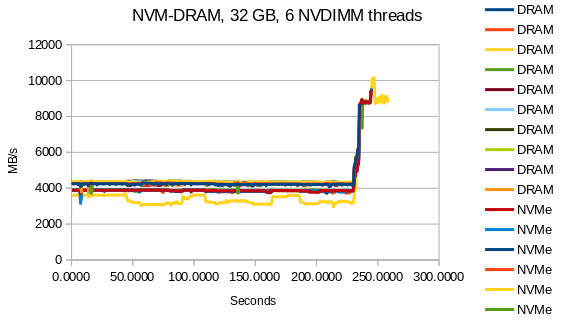
\includegraphics[scale=0.7]{Benchmarks/NVM-DRAM_32GB_6_Thread.png}
%\caption{NVM-DRAM, 32 GB, 6 NVDIMM Threads}
%\label{fig:NVM_DRAM_sec}
%\end{figure}

\begin{figure}[!hbtp]
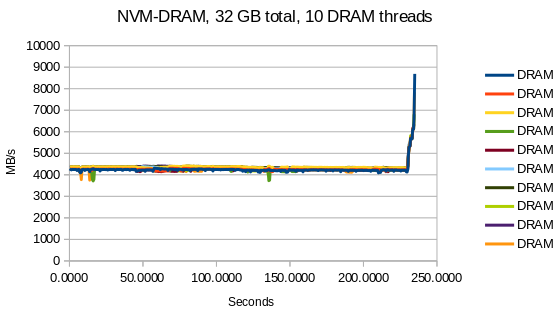
\includegraphics[scale=0.7]{Benchmarks/NVM-DRAM_32GB_10_DRAM_Threads.png}
\caption{DRAM threads in this figure and NVDIMM threads in figure \ref{fig:NVM_DRAM_sec2} competing for bandwidth over a certain time period. Threads ends at different times.}
\label{fig:NVM_DRAM_sec1}
\end{figure}

\begin{figure}[!hbtp]
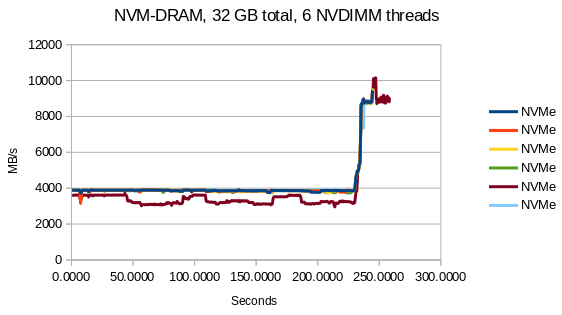
\includegraphics[scale=0.7]{Benchmarks/NVM-DRAM_32GB_6_NVDIMM_Threads.png}
\caption{DRAM threads in figure \ref{fig:NVM_DRAM_sec1} and NVDIMM threads in this figure competing for bandwidth over a certain time period. Threads ends at different times.}
\label{fig:NVM_DRAM_sec2}
\end{figure}

\pagebreak
\subsubsection{DRAM-NVM}
\label{section:DRAM-NVM}
In this version of the benchmark there will be one group of threads that transfer data from a DRAM array to a DRAM array and another group of threads that will transfer data from a DRAM array to a NVDIMM array. This code only have one difference when compared to the code in \ref{section:NVM-DRAM}. The difference is found in line 51-61 where data is transferred from DRAM-NVDIMM insted of from NVDIMM-DRAM.

\begin{lstlisting}[caption={DRAM-NVM source code},escapeinside={{/*!}{!*/}}]
#pragma omp parallel
{
	int thread_id = omp_get_thread_num();
	int i,j;
	double *drm_read_array;
	double *drm_write_array;
	TOID(double) nvm_write_array;
	srand((unsigned int)time(NULL));
	#pragma omp master
	{
		/* Creates array where the test result will be added. */
	}
	//Creates all the arrays needed for the test.
	#pragma omp barrier
	if(thread_id < totalThreads-nvmThreads){
		drm_read_array = (double*)malloc(ARRAY_LENGTH*sizeof(double));
    	drm_write_array = (double*)malloc(ARRAY_LENGTH*sizeof(double));
		#pragma omp critical
		{
			for(i=0;i<ARRAY_LENGTH;i++){
				drm_read_array[i] = ((double)rand()/(double)(RAND_MAX));
				drm_write_array[i] = ((double)rand()/(double)(RAND_MAX));
			}
		}
	}
	else if(thread_id >= totalThreads-nvmThreads){
		drm_read_array = (double*)malloc(ARRAY_LENGTH*sizeof(double));
    	POBJ_ALLOC(pop, &nvm_write_array, double, sizeof(double) * ARRAY_LENGTH, NULL, NULL);
		#pragma omp critical
		{
			for(i=0;i<ARRAY_LENGTH;i++){
				drm_read_array[i] = ((double)rand()/(double)(RAND_MAX));
				D_RW(nvm_write_array)[i] = ((double)rand()/(double)(RAND_MAX));
			}
		}
	}
	//Doing the test.
	#pragma omp barrier
	if(thread_id < totalThreads-nvmThreads){
		//From DRAM to DRAM:
		for(i=0;i<total_tests;i++){
			//Time start
			test_time[thread_id][i] = mysecond();	
			for(j=0;j<ARRAY_LENGTH;j++){
				drm_write_array[j] = drm_read_array[j];
			}
			//Time stop.
			test_time[thread_id][i] = mysecond() - test_time[thread_id][i];
		}
	}
	else if(thread_id >= totalThreads-nvmThreads){
		//From DRAM to NVM:
		for(i=0;i<total_tests;i++){
			//Time start
			test_time[thread_id][i] = mysecond();
			for(j=0;j<ARRAY_LENGTH;j++)
				D_RW(nvm_write_array)[j] = drm_read_array[j];		
			//Time stop.
			test_time[thread_id][i] = mysecond() - test_time[thread_id][i];
		}
	}
	else
		printf("ERROR\n");
	/* Freeing up DRAM and NVDIMM arrays */
}
\end{lstlisting}

%\clearpage
\begin{table}[!hbtp]
\centering
\begin{tabular}{ |c|c|c|c|c| }
\hline
DRAM & NVDIMM & & & \\
threads & threads & DRAM & NVDIMM & Sum \\
\hline
15 & 1 & 61002.60 & 3581.48 & 64584.09 \\
\hline
14 & 2 & 56598.08 & 7323.96 & 63922.04 \\
\hline
13 & 3 & 53247.52 & 10954.06 & 64201.58 \\
\hline
12 & 4 & 48681.71 & 15070.61 & 63752.32 \\
\hline
11 & 5 & 44761.80 & 18725.90 & 63487.70 \\
\hline
10 & 6 & 41022.39 & 22614.45 & 63636.84 \\
\hline
9 & 7 & 36897.42 & 26557.71 & 63455.13 \\
\hline
8 & 8 & 32548.18 & 30570.88 & 63119.07 \\
\hline
7 & 9 & 28892.06 & 33996.95 & 62889.00 \\
\hline
6 & 10 & 24941.87 & 38191.10 & 63132.97 \\
\hline
5 & 11 & 20563.14 & 42263.28 & 62826.42 \\
\hline
4 & 12 & 16803.83 & 45915.39 & 62719.21 \\
\hline
3 & 13 & 12648.47 & 49341.90 & 61990.38 \\
\hline
2 & 14 & 8386.48 & 53331.10 & 61717.57 \\
\hline
1 & 15 & 4189.43 & 57348.14 & 61537.57 \\
\hline
\end{tabular}
\caption{DRAM-NVM, 32 GB total. DRAM and NVDIMM threads competing for bandwidth. Speed are in MB/s.}
\label{tab:DRAM_NVM}
\end{table}

The result of this benchmark is shown in figure \ref{fig:DRAM_NVM} and table \ref{tab:DRAM_NVM}. The result in figure \ref{fig:DRAM_NVM} is similar to the result in figure \ref{fig:NVM_DRAM} where NVDIMM speed increases and DRAM speed decreases at the same around the same rate. The sum of DRAM and NVDIMM speed remains stable at around 63,000 MB/s. Only at eleven NVDIMM threads and higher does the speed decrease a little. 

\begin{figure}[!hbtp]
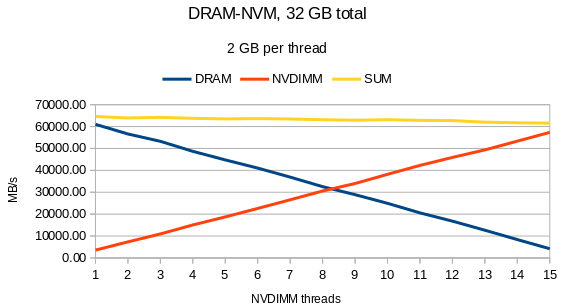
\includegraphics[scale=0.7]{Benchmarks/DRAM-NVM_32GB_Figure.png}
\caption{Graph of table \ref{tab:DRAM_NVM}. DRAM and NVDIMM threads competing for bandwidth.}
\label{fig:DRAM_NVM}
\end{figure}
%\clearpage
%\pagebreak
%New graphs with second on x-axis and bandwidth on Y-axis. 500 iterations.
Figure \ref{fig:DRAM_NVM_sec1} and \ref{fig:DRAM_NVM_sec2} shows the result of the same benchmark as figure \ref{fig:DRAM_NVM}, but with second on the x-axis instead of NVDIMM threads. Figure  \ref{fig:DRAM_NVM} has been split in two in order to make it more readable, figure \ref{fig:DRAM_NVM_sec1} shows all the DRAM and figure \ref{fig:DRAM_NVM_sec2} shows all the NVDIMM threads.
%Similar to the other two benchmarks the DRAM threads in Figure \ref{fig:DRAM_NVM_sec} have more consistent speed than the NVDIMM. 
Unlike the other two benchmarks the DRAM threads in Figure \ref{fig:DRAM_NVM_sec1} have less consistent speed than the DRAM in the benchmarks, this might be because both group of threads are reading from DRAM.
The speed of the DRAM threads is around 4,100 MB/s until the end where it increases sharply because other threads have completed their tasks and given the remaining threads more bandwidth. The speed of the NVDIMM is more unstable. The speed remains at 3,800 MB/s, but all of the NVDIMM threads drop their speed several time during the test. Sometimes as low as 1,900 MB/s.

%\begin{figure}[!hbtp]
%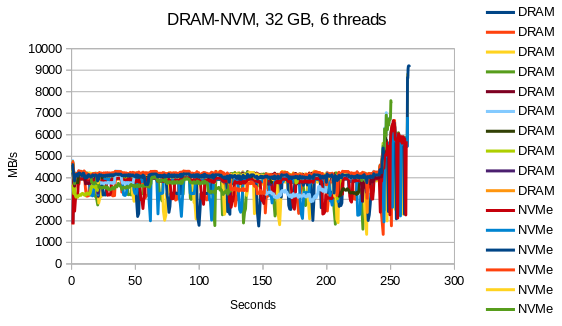
\includegraphics[scale=0.7]{Benchmarks/DRAM-NVM_32GB_6_Thread.png}
%\caption{DRAM-NVM, 32 GB, 6 NVDIMM Threads}
%\label{fig:DRAM_NVM_sec}
%\end{figure}

\begin{figure}[!hbtp]
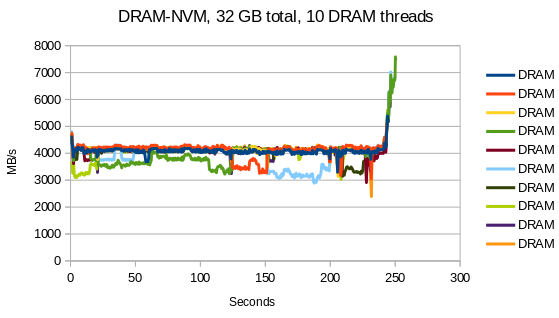
\includegraphics[scale=0.7]{Benchmarks/DRAM-NVM_32GB_10_DRAM_Threads.png}
\caption{DRAM threads in this figure and NVDIMM threads in figure \ref{fig:DRAM_NVM_sec2} competing for bandwidth over a certain time period. Threads ends at different times.}
\label{fig:DRAM_NVM_sec1}
\end{figure}

\begin{figure}[!hbtp]
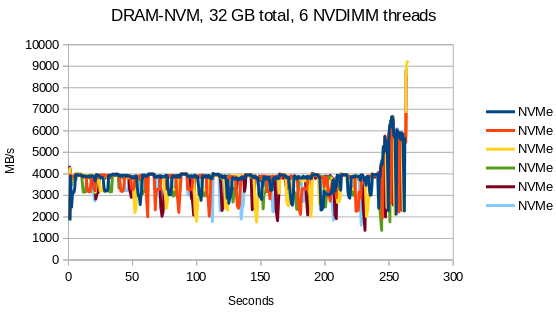
\includegraphics[scale=0.7]{Benchmarks/DRAM-NVM_32GB_6_NVDIMM_Threads.png}
\caption{DRAM threads in figure \ref{fig:DRAM_NVM_sec1} and NVDIMM threads in this figure competing for bandwidth over a certain time period. Threads ends at different times.}
\label{fig:DRAM_NVM_sec2}
\end{figure}

\pagebreak
\subsubsection{Observations}
\label{section:Observations}
The benchmarks at section \ref{section:NVM-DRAM} and section \ref{section:DRAM-NVM} have result more similar than the result in chapter \ref{section:NVM-NVM}. This is because the transfer speed DRAM to NVDIMM and NVDIMM to DRAM is almost identical. The DRAM-NVDIMM speed with one thread is 3581 MB/s and with fifteen thread the speed is 57348 MB/s. The NVDIMM-DRAM speed with one thread is 3742 an with fifteen thread the speed is 60031 MB/s. The speed with one and fifteen threads are almost the same. The rate the speed increase for each NVDIMM are also very similar.

The speed of the NVDIMM to NVDIMM in section \ref{section:NVM-NVM} is slower than the other two benchmarks. When there are five threads the total speed of both DRAM and NVDIMM starts to decrease and at fifteen threads the total speed has decreased by 10,000 MB/s. 
This means that if a program has two group of threads, one group only working on DRAM and the other only in NVDIMM. The program should not have more than five threads working on NVDIMM if the objective is to maximize performance.

Figure \ref{fig:NVM_NVM_sec} in section \ref{section:NVM-NVM} and figure \ref{fig:DRAM_NVM_sec2} in section \ref{section:DRAM-NVM} shows the NVDIMM threads fluctuate a lot. The figure \ref{fig:NVM_DRAM_sec2} in section \ref{section:NVM-DRAM} on the other hand show that all the NVDIMM threads except for one is a lot more stable. This might mean that writing to NVDIMM is a lot more sensitive to disturbances than what reading data from NVDIMM is.

The NVDIMM Stream in section \ref{section:STREAM_NVDIMM} is also similar where there are only NVDIMM threads and no traffic on DRAM. When each thread have their own core there is a smooth increase from one thread to sixteen threads. But when the hyper-treads are included and there are more than one thread per core the speed starts to fluctuate up and down for each new thread that is included.

Regardless of what the reason is for the fluctuations. The fluctuation might make it difficult to predict how much time it takes for an NVDIMM thread to complete a task.

%fra conclusion.
Table \ref{tab:Q1} show the copy speed of the two Stream benchmarks mentioned above. Table \ref{tab:Q1} end at sixteen threads while the Stream benchmarks test up to 32 threads. This is because the NVDIMM fluctuate too much to find a pattern. When the Stream is testing speed of only one thread the NVDIMM have a performance of 43\% of the speed of DRAM. When the number of threads increases the difference remain at around 40\% up until six threads. The exception to this is the test with two threads where the NVDIMM performance is 52\% of the DRAM performance.
The performance of NVDIMM at seven threads is at 51\% and when the number of threads increases the performance increases and end at 75\% when there is sixteen threads.

The reason the performance increases as more threads are added is because DRAM at 65,000 MB/s have reached the maximum capacity of the memory bandwidth. This allows the NVDIMM threads to catch up with the DRAM performance, but NVDIMM is only able to reach a performance 75\% of DRAM.

\begin{table}[!hbtp]
\centering
\begin{tabular}{ |c|c|c|c| }
\hline
Threads & DRAM & NVDIMM & Difference in \%\\
\hline
1 & 11673.5 & 5036.7 & 43.1 \\
\hline
2 & 22995.1 & 11970.2 & 52.1 \\
\hline
3 & 33554.9 & 12715.1 & 37.9 \\
\hline
4 & 42917.3 & 16349.6 & 38.1 \\
\hline
5 & 50260.9 & 20935.0 & 41.7 \\
\hline
6 & 53612.5 & 23119.7 & 43.1 \\
\hline
7 & 56100.8 & 28694.5 & 51.1 \\
\hline
8 & 58554.6 & 32104.6 & 54.8 \\
\hline
9 & 60491.7 & 37491.8 & 62.0 \\
\hline
10 & 62242.2 & 41394.8 & 66.5 \\
\hline
11 & 64257.1 & 44856.8 & 69.8 \\
\hline
12 & 64890.3 & 44695.1 & 68.9 \\
\hline
13 & 65648.8 & 47377.9 & 72.2 \\
\hline
14 & 65606.5 & 48853.3 & 74.5 \\
\hline
15 & 65665.5 & 51273.9 & 78.1 \\
\hline
16 & 65509.8 & 48704.8 & 74.3 \\
\hline
\end{tabular}
\caption{Difference in STREAM performance between DRAM and NVDIMM. Speeds are in MB/s.}
\label{tab:Q1}
\end{table}

The results from some of these benchmarks will be used in later chapter in order to make a prediction of how long it will take to complete a certain task. 

\clearpage
\section{DRAM and NVDIMM Cooperation}
\label{Chapter:Cooperation}
\subsection{Introduction}
%The size of data that must be analyzed keeps increasing year after year and the prize for DRAM are not getting cheaper. NVDIMM offer a lot of storage at a cheaper prize. 
There are instances where data become too large to be stored in DRAM and some of the data must be offloaded to NVDIMM. The data can be analyzed on NVDIMM just like it was on DRAM.
%This opens the opportunity to offload some of the data to the NVDIMM where the data will be analyzed the same way as the data on the DRAM. 
The downside to this strategy is that NVDIMM is slower than DRAM so the question is how much data can be offloaded to NVDIMM. If the user offloads too much data to NVDIMM then the threads working on analyzing the data on DRAM will be idle while waiting for NVDIMM threads to complete.

The goal of this chapter is to find a formula that will make it possible to estimate how much data should be offloaded to NVDIMM. By using the the formula with different combination of DRAM and NVDIMM the user can choose how many threads that should be allocated to NVDIMM.

There are two versions of the code that are being used. They have been programmed slightly differently in the way data is read. This is to explore which of them is the fastest.

%The goal is to find a formula that can easily calculate how much data can be offloaded to the NVDIMM from DRAM. The time taken to perform calculation on NVDIMM must be equal to the amount of time it takes to run calculation on the remaining data on DRAM. 

\subsection{Calculation of NVDIMM part}
\subsubsection{Explanation of formula}
In order to use the formula one must measure the NVDIMM and DRAM speed using the benchmark shown in section \ref{section:NVM-NVM} because in this chapter DRAM threads will transfer data to and from DRAM and NVIDMM threads will transfer data to and from NVDIMM. This is also what are being done in the benchmark I have chosen.
%made in a previous chapter where speed was measured when data was transferred from DRAM to DRAM and from NVDIMM to NVDIMM simultaneously with different amount threads allocated to the different processes. 
By using the speed from the benchmark in the formula below along with the size of the data that will be used in the calculation the user can easily calculate how much data can be transferred to NVDIMM before DRAM complete its task before NVDIMM. The formula does only decide how much data can be allocated to NVDIMM with a certain amount of threads. This means that the user must probably use the formula several times where the number of NVDIMM threads varies from one to five in order to find a combination of threads and data allocated to NVDIMM that the user is satisfied with. 

\begin{equation}
    \frac{Total\_data-nvdimm\_data}{dram\_speed} = \frac{nvdimm\_data}{nvdimm\_speed}
\end{equation}
\begin{equation}
    nvdimm\_data = \frac{nvdimm\_speed*Total\_data}{nvdimm\_speed+dram\_speed}
\end{equation}

%\caption{The formula used to decide how much should be allocated to NVDIMM.}
%\label{fig:mathFormula} \[ \]

I have created a program that will test this formula to see if it is accurate.
This program has an two dimensional array filled with data. The program starts at element (1,1) of the array where it add together all of its eight neighbors and then takes the average. The result is stored in the same position in another two dimensional array. The program does this for every element between (1,1) and (m-2,n-2), m and n is the length of the 2D array used by the program. 
The program repeats this process ten times and after each time the program will swap the DRAM arrays and NVDIMM array. The time is measured at the beginning of the process and at the end, this time is called total\_time in the code.
Each thread will also measure the time it takes to complete their own tasks, in the code this is called individual\_time.

Listing \ref{lst:LABserial} is an example of the serial code of the program. The array has not been divided into two.
The thread will repeat the while-loop on line 1 k\_length which is ten times. It will start the time measurement at line 2. From line 3-10 the thread will pass through the the 2D-array row by row starting from element (1,1) and end at element (m-2,n-2). At each element the thread will calculate the average of all the elements neighbors, eight neighbors in total.
The thread will then stop the time measurement at line 11 and swap the arrays at line 12-14.
It will also increase k by one and start over if k is still lower than k\_length.

\begin{lstlisting}[caption={Serial code that will be used in the first and second versions.}, label={lst:LABserial}]
while(k<K_length){
	total_time[k] = mysecond();
	for( i=1; i<m-2; i++){
		for( j=1; j<n-2; j++){
			temp =  A[i-1][j-1] + A[i-1][j] + A[i-1][j+1]+
					    A[i][j-1]        +        A[i][j+1]+
					    A[i+1][j-1] + A[i+1][j] + A[i+1][j+1];
			B[i][j] = temp/8;
		}
	}
	total_time[k] = mysecond() - total_time[k];
	temp_array = A;
	A = B;
	B = temp_array;
	k++;
}
\end{lstlisting}

\subsubsection{Distribution}
By using the formula described above we have calculated the distribution of data between DRAM and NVDIMM in table \ref{tab:distribution16GB} and \ref{tab:distribution160GB}. The tables show the number of NVDIMM threads assigned in first column. Second and third columns show the speed of DRAM and NVDIMM. The speed is from the result of the benchmark in section \ref{section:NVM-NVM}. Fourth column shows how much data should be placed on NVDIMM. This is based on the formula described previously in this chapter. The last column shows how many rows in the 2D array of data must be delegated to NVDIMM in order for the size of the array to be close to the previous column. Table \ref{tab:distribution16GB} show how many rows in a 2d-array where m and n are 31,623 elements should be delegated to NVDIMM. Table \ref{tab:distribution160GB} is the same, but here m and n are 100,000 elements

\begin{table}[!hbtp]
\centering
\begin{tabular}{ |c|c|c|c|c| } 
\hline
NVM & Aggregate DRAM  & Aggregate NVDIMM & NVDIMM & NVDIMM \\
Threads & bandwidth in MB/s & bandwidth in MB/s &in MB/s & rows \\
\hline
1 & 61042.84 & 3038.16 & 379.30 & 750 \\
\hline
2 & 57761.80 & 6027.24 & 755.91 & 1494 \\
\hline
3 & 53767.10 & 9223.43 & 1171.42 & 2315 \\
\hline
4 & 51257.79 & 12630.42 & 1581.59 & 3126 \\
\hline
5 & 47770.89 & 15202.48 & 1931.32 & 3817 \\
\hline
\end{tabular}
\caption{Distribution of 16 GB data between DRAM and NVDIMM. Both m and n are 31,623 elements.}
\label{tab:distribution16GB}
\end{table}

\begin{table}[!hbtp]
\centering
\begin{tabular}{ |c|c|c|c|c| } 
\hline
NVM & Aggregate DRAM  & Aggregate NVDIMM & NVDIMM & NVDIMM \\
Threads & bandwidth in MB/s & bandwidth in MB/s &in MB/s & rows \\
\hline
1 & 61042.84 & 3038.16 & 3792.90 & 2371 \\
\hline
2 & 57761.80 & 6027.24 & 7558.96 & 4724 \\
\hline
3 & 53767.10 & 9223.43 & 11714.05 & 7321 \\
\hline
4 & 51257.79 & 12630.42 & 15815.65 & 9885 \\
\hline
5 & 47770.89 & 15202.48 & 19312.90 & 12071 \\
\hline
\end{tabular}
\caption{Distribution of 160 GB data between DRAM and NVDIMM. Both m and n are 100,000 elements.}
\label{tab:distribution160GB}
\end{table}

%Distribution of m\\
%\subsection{Prediction}
\subsubsection{Prediction}
The distributions calculated in the previous section are used in this section to predict how much time DRAM and NVDIMM will take to complete their tasks.
The first column shows the number of NVDIMM threads. Second and fifth columns show the speed of DRAM and NVDIMM, they are also from the result of the benchmark in section \ref{section:NVM-NVM}.
Third and sixth columns show how much data is allocated to DRAM and NVDIMM. Fourth and seventh columns show the how much time it takes for DRAM and NVDIMM to complete their tasks.

\begin{table}[!hbtp]
\centering
\begin{tabular}{ |c|c|c|c|c|c|c| }
\hline
        & DRAM  & DRAM & DRAM      & NVDIMM & NVDIMM & NVDIMM \\
Threads & speed & Size & pred.time & speed  & Size   & pred.time \\
\hline
1 & 61042.84 & 15241.41 & 0.2497 & 3038.16 & 758.59 & 0.2497 \\
\hline
2 & 57761.80 & 14488.19 & 0.2508 & 6027.24 & 1511.81 & 0.2508 \\
\hline
3 & 53767.10 & 13657.16 & 0.2540 & 9223.43 & 2342.84 & 0.2540 \\
\hline
4 & 51257.79 & 12836.82 & 0.2504 & 12630.42 & 3163.18 & 0.2504 \\
\hline
5 & 47770.89 & 12137.37 & 0.2541 & 15202.48 & 3862.63 & 0.2541 \\
\hline
\end{tabular}
\caption{Time prediction with 16 GB of data.Both m and n are 31,623 elements.}
\label{tab:Prediction16GB}
\end{table}

\begin{table}[!hbtp]
\centering
\begin{tabular}{ |c|c|c|c|c|c|c| }
\hline
        & DRAM  & DRAM & DRAM      & NVDIMM & NVDIMM & NVDIMM \\
Threads & speed & Size & pred.time & speed  & Size   & pred.time \\
\hline
1 & 61042.84 & 152414.20 & 3.7453 & 3038.16 & 7585.80 & 3.7453 \\
\hline
2 & 57761.80 & 144882.07 & 3.7624 & 6027.24 & 15117.93 & 3.7624 \\
\hline
3 & 53767.10 & 136571.90 & 3.8101 & 9223.43 & 23428.10 & 3.8101 \\
\hline
4 & 51257.79 & 128368.69 & 3.7566 & 12630.42 & 31631.31 & 3.7566 \\
\hline
5 & 47770.89 & 121374.21 & 3.8111 & 15202.48 & 38625.79 & 3.8111 \\
\hline
\end{tabular}
\caption{Time prediction with 160 GB of data.Both m and n are 100,000 elements.}
\label{tab:Prediction160GB}
\end{table}

\begin{comment}
\begin{table}[!hbtp]
\centering
\begin{tabular}{ |c|c|c|c|c|c|c| } 
\hline
        & DRAM  & DRAM & DRAM      & NVDIMM & NVDIMM & NVDIMM \\
Threads & speed & Size & pred.time & speed  & Size   & pred.time \\
\hline
1 & 61042.84 & 15620.75 & 0.2559 & 3038.16 & 379.48 & 0.1249 \\
\hline
2 & 57761.80 & 15244.31 & 0.2639 & 6027.24 & 755.92 & 0.1254 \\
\hline
3 & 53767.10 & 14828.91 & 0.2758 & 9223.43 & 1171.32 & 0.1270 \\
\hline
4 & 51257.79 & 14418.57 & 0.2813 & 12630.42 & 1581.66 & 0.1252 \\
\hline
5 & 47770.89 & 14068.95 & 0.2945 & 15202.48 & 1931.28 & 0.1270 \\
\hline
\end{tabular}
\caption{Prediction, 16 GB}
\label{tab:Prediction16GB}
\end{table}
\begin{table}[!hbtp]
\centering
\begin{tabular}{ |c|c|c|c|c|c|c| }
\hline
 & DRAM & DRAM & DRAM & NVDIMM & NVDIMM & NVDIMM \\
Threads & speed & Size & pred.time & speed & Size & pred.time \\
\hline
1 & 61042.84 & 156206.40 & 3.8384 & 3038.16 & 3793.60 & 1.8730 \\
\hline
2 & 57761.80 & 152441.60 & 3.9587 & 6027.24 & 7558.40 & 1.8811 \\
\hline
3 & 53767.10 & 148286.40 & 4.1369 & 9223.43 & 11713.60 & 1.9050 \\
\hline
4 & 51257.79 & 144184.00 & 4.2194 & 12630.42 & 15816.00 & 1.8783 \\
\hline
5 & 47770.89 & 140686.40 & 4.4175 & 15202.48 & 19313.60 & 1.9056 \\
\hline
\end{tabular}
\caption{Prediction, 160 GB}
\label{tab:Prediction160GB}
\end{table}
\end{comment}

\subsection{First program version}
There are two groups of threads that work in parallel in this program. The first group of threads works on the part of the data that is stored on DRAM and the other works on the data stored on NVDIMM. 
One thread in each group works on data that borders with the other group. In the DRAM group that is the thread with the highest thread\_id. Each of the elements in the last row of data will have three neighbors that exist on the NVDIMM side. This means that the thread must access the NVDIMM in order to get the data. The NVDIMM thread with the lowest thread\_id also has elements in the first row of data that have three neighbours that exist in DRAM that must be accessed by the thread directly.
%\\
%\\
%Explaination of code:\\

Listing \ref{lst:FirstVersion} only shows the calculation process, it does not show the rest of the code. Allocation of memory has been done by all the threads, as a result the data have been spread across all the memory channels. 
The data is a 2d array where the rows of data on DRAM will be divided equally between the DRAM threads, the rows of data on NVDIMM will also be divided equally between the NVDIMM threads. The variable slice\_start contains the index of the row where the tread must start at and slice\_end holds the index of the row the thread must stop at.
Array A and B are DRAM arrays and array C and D are NVDIMM arrays. The average found by adding together eight neighbors in A will be placed in same position in B. The same is true for C and D.

The process is repeated K\_length time, usually ten times in my tests.
The code measures the time taken to complete one iteration of calculation, this is done in the beginning of the code at line 5 and at the end at line 84 by a single thread.
All the threads then get divided into the DRAM and NVDIMM at line 8. If the thread\_id of a thread is less than the dram\_threads is it will do calculation on the data in DRAM, the rest will fail the if test and move on to the else bracket at line 42. Dram\_threads is the total amount of threads that will be working on data in DRAM.

At line 11 the thread with the highest thread\_id will pass the if test and the rest will move on to line 30. The thread with highest thread\_id will then measure time at line 12 and end the measurement in line 29, this is the start and the end of the bracket. The thread will then enter a double for-loop at line 13-20 that will go through elements from position (slice\_start,1) until (slice\_end-1,n-1), this leaves out the last row assigned to the tread, that row will be dealt with later. At each element the for-loop it will add all of its eight neighbors together at line 15-17 and divide by eight at line 18.
The thread will then enter a new for-loop at line 23, this for-loop will calculate average of the last row on DRAM. Elements of this row have three neighbors that exist in NVDIMM. The thread will access the NVDIMM directly when adding the eight neighbors at line 24-26. Data on NVDIMM are accessed by the thread at line 26.

For all the other DRAM threads that jumped to line 30 will start by taking time measurement at the beginning and at the end of the bracket at line 31 and 40. The code from line 32-39 is identical to line 13-20 described before.

The group of NVDIMM enters the else bracket at line 42 where the thread with the lowest thread\_id will pass the if-sentence at line 44, the rest will move on to the else bracket at line 62. The thread will then measure time at line 45 and end the measurement in line 61.
It will then enter a for-loop at line 47 and will begin calculating the average of the neighbors of the elements in the first row. The first row has three of its eight neighbors in the row above and they exist in the DRAM.
Once done the thread will move on to a new for-loop at line 53. This for-loop will go through the rest of the portion of data the thread has been given and calculate the average of each elements neighbors.

The rest of the NVDIMM threads will move into the else bracket at line 62. The code here is very similar to the code at 31-40 that has been described at a previous paragraph. The only difference is that the code at line 66-68 reads from NVDIMM instead DRAM.

All the threads will wait a barrier at line 75 until all threads are done. After that one thread will enter a single bracket where array A and B will swap places, array C and D will also swap places. The time it took for this one iteration will be registered at line 84. After this the code will move back to line 1.


\begin{lstlisting}[caption={First version of the code where the threads will access data on the other memory type directly.},escapeinside={{/*!}{!*/}}, label={lst:FirstVersion}]
while(k<K_length){
	#pragma omp barrier
	#pragma omp single
	{
		total_time[k] = mysecond();
	}
	//Divides threads into DRAM threads and NVDIMM threads.
	if( thread_id < dram_threads ){

		//for the thread bordering on NVDIMM thread.
		if( thread_id==(dram_threads-1) ){
			individual_time[k][thread_id] = mysecond();
			for( i=slice_start; i<slice_end-1; i++){
				for( j=1; j<nMinusOne; j++){
					temp = A[i-1][j-1] + A[i-1][j] + A[i-1][j+1]+
						   A[i][j-1]        +        A[i][j+1]+
					       A[i+1][j-1] + A[i+1][j] + A[i+1][j+1];
					B[i][j] = temp*inverseEigth;
				}
			}
			
			i = slice_end-1;
			for( j=1; j<nMinusOne; j++){
				temp = A[i-1][j-1] + A[i-1][j] + A[i-1][j+1]+
					    A[i][j-1]        +        A[i][j+1]+
				       D_RO(C)[i*n+j] + D_RO(C)[i*n+j] + D_RO(C)[i*n+j];
				B[i][j] = temp*inverseEigth;
      		}
			individual_time[k][thread_id] = mysecond() - individual_time[k][thread_id];
		}else{
			individual_time[k][thread_id] = mysecond();
			for( i=slice_start; i<slice_end; i++){
				for( j=1; j<nMinusOne; j++){
					temp = A[i-1][j-1] + A[i-1][j] + A[i-1][j+1]+
						   A[i][j-1]        +        A[i][j+1]+
						   A[i+1][j-1] + A[i+1][j] + A[i+1][j+1];
					B[i][j] = temp*inverseEigth;
				}
			}
			individual_time[k][thread_id] = mysecond() - individual_time[k][thread_id];
		}
	}else{
		//for the thread bordering on DRAM thread.
		if( thread_id==dram_threads ){
			individual_time[k][thread_id] = mysecond();
			i=0;
			for( j=1; j<nMinusOne; j++){
				temp = A[dram_part-1][j-1]+A[dram_part-1][j]+A[dram_part-1][j+1]+
					   D_RO(C)[i*n+(j-1)]            +            D_RO(C)[i*n+(j+1)]+
					   D_RO(C)[(i+1)*n+(j-1)] + D_RO(C)[(i+1)*n+j] + D_RO(C)[(i+1)*n+(j+1)];
				D_RW(D)[i*n+j] = temp*inverseEigth;
			}
			for( i=slice_start+1; i<slice_end-1; i++){
				for( j=1; j<nMinusOne; j++){
					temp = D_RO(C)[(i-1)*n+(j-1)] + D_RO(C)[(i-1)*n+j] + D_RO(C)[(i-1)*n+(j+1)]+
						   D_RO(C)[i*n+(j-1)]            +            D_RO(C)[i*n+(j+1)]+
						   D_RO(C)[(i+1)*n+(j+1)] + D_RO(C)[(i+1)*n+j] + D_RO(C)[(i+1)*n+(j+1)];
					D_RW(D)[i*n+j] = temp*inverseEigth;
				}
			}
			individual_time[k][thread_id] = mysecond() - individual_time[k][thread_id];
		}else{
			individual_time[k][thread_id] = mysecond();
			for( i=slice_start; i<slice_end; i++){
				for( j=1; j<nMinusOne; j++){
					temp = D_RO(C)[(i-1)*n+(j-1)] + D_RO(C)[(i-1)*n+j] + D_RO(C)[(i-1)*n+(j+1)]+
						   D_RO(C)[i*n+(j-1)]            +            D_RO(C)[i*n+(j+1)]+
						   D_RO(C)[(i+1)*n+(j-1)] + D_RO(C)[(i+1)*n+j] + D_RO(C)[(i+1)*n+(j+1)];
                    D_RW(D)[i*n+j] = temp*inverseEigth;
				}
			}
			individual_time[k][thread_id] = mysecond() - individual_time[k][thread_id];
		}
	}
	#pragma omp barrier
	#pragma omp single
	{
		tempArray = B;
        B=A;
        A=tempArray;
		temp_nvdimm = C;
		C = D;
		D = temp_nvdimm;
		total_time[k] = mysecond() - total_time[k];
		k++;
	}
	#pragma omp barrier
}//End of while
\end{lstlisting}


In table \ref{tab:FirstVersion16GB} and \ref{tab:FirstVersion160GB} the first two columns show m and n which is the length of the 2D-array. Third columns show how many rows are assigned to NVDIMM. Fourth and fifth column shows the number of DRAM and NVDIMM threads the test have used.
Columns five and six show the time it takes for DRAM and NVDIMM to complete their tasks. Column seven show the total time for the test.

Each row in table \ref{tab:FirstVersion16GB} and \ref{tab:FirstVersion160GB} is the result of running the code shown above one time. The code is running its test ten times and all threads measure the time to complete their own tasks. The slowest DRAM thread and slowest NVDIMM thread in each test gets stored. The time shown in column six and seven is the average of those times. Total time in column eight is the average time it takes for all the threads to complete.

\begin{table}[!hbtp]
\centering
\begin{tabular}{ |c|c|c|c|c|c|c|c| }
\hline
&  & NVDIMM & DRAM & NVDIMM & DRAM & NVDIMM & Total \\
M & N & rows & threads & threads & time & time & time \\
\hline
31623 & 31623 & 750 & 15 & 1 & 0.3099 & 0.3431 & 0.3457 \\
\hline
31623 & 31623 & 1494 & 14 & 2 & 0.3117 & 0.3416 & 0.3427 \\
\hline
31623 & 31623 & 2315 & 13 & 3 & 0.2937 & 0.3522 & 0.3542 \\
\hline
31623 & 31623 & 3126 & 12 & 4 & 0.2882 & 0.3571 & 0.3578 \\
\hline
31623 & 31623 & 3817 & 11 & 5 & 0.2900 & 0.3510 & 0.3512 \\
\hline
\end{tabular}
\caption{Result of the first version of the code with 16 GB of data.}
\label{tab:FirstVersion16GB}
\end{table}
\begin{figure}[!hbtp]
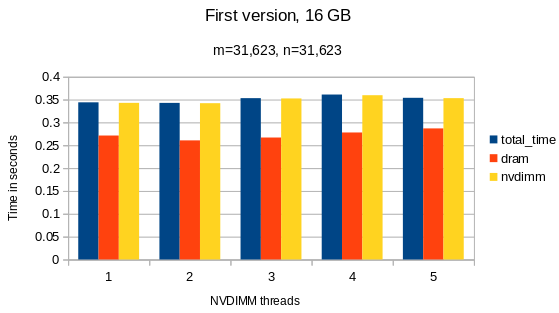
\includegraphics[scale=0.7]{Large_Array_test/First_version_16GB.png}
\caption{Result of the first version of the code with 16 GB of data in graph form.}
\label{fig:FirstVersion16GB}
\end{figure}

The DRAM times of the in table \ref{tab:FirstVersion16GB} are almost matching the predicted times in table \ref{tab:Prediction16GB}. The difference between predicted time and actual time is at most 0.05 seconds.
When comparing the predicted DRAM time in table \ref{tab:Prediction160GB} and actual DRAM time in table \ref{tab:FirstVersion160GB} one can see that predicted time is very close to actual time. The biggest difference is when there are four NVDIMM threads. With four NVDIMM threads the difference is 0.24 seconds.

The NVDIMM time predictions are a lot worse. According to the prediction the DRAM and NVDIMM are supposed to complete at the same time, but this is not happening. When comparing the predicted time for NVDIMM in table \ref{tab:FirstVersion16GB} with the measured time in table \ref{tab:Prediction16GB} one can see that NVDIMM takes a lot longer time to complete. NVDIMM used about 0.1 second longer to complete its tasks, this is about 30\% longer than predicted time.
The difference becomes even greater when the size of the array increases. The NVDIMM predicted time in table \ref{tab:Prediction160GB} is in the range of between 3.74 and 3,81 seconds depending on how many threads are given to NVDIMM. The time it takes for NVDIMM to complete their task is almost twice as long for all the tests.

Since the time prediction for the DRAM was accurate this should mean that there isn't anything wrong with the prediction. The NVDIMM has performed slower than expected based on the benchmarks collected in section \ref{section:NVM-NVM}.

The total time in table \ref{tab:FirstVersion16GB} is almost identical to the NVDIMM. This makes sense because the only thing happening when the threads are not doing their tests is the swapping of arrays and this takes almost no time at all. Since the slowest thread is always an NVDIMM then the total time should be equal to the NVDIMM time.

This is not the case however in the table \ref{tab:FirstVersion160GB}. Total time in this result is only once identical to the NVDIMM time and that is when NVDIMM is given five threads. For all the other total times there are a time difference of between 0.5 and 2 seconds. 
Based on the code the total time should be identical to NVDIMM time like the result in table \ref{tab:FirstVersion16GB} was. The only difference between these results is that the arrays are bigger, but that should not affect the time it take to swap arrays. 

\begin{table}[!hbtp]
\centering
\begin{tabular}{ |c|c|c|c|c|c|c|c| }
\hline
&  & NVDIMM & DRAM & NVDIMM & DRAM & NVDIMM & Total \\
M & N & rows & threads & threads & time & time & time \\
\hline
100000 & 100000 & 2371 & 15 & 1 & 3.7423 & 4.4166 & 6.1124 \\
\hline
100000 & 100000 & 4724 & 14 & 2 & 4.0061 & 5.0799 & 7.1181 \\
\hline
100000 & 100000 & 7321 & 13 & 3 & 4.0294 & 7.3525 & 7.8412 \\
\hline
100000 & 100000 & 9885 & 12 & 4 & 4.0449 & 6.2484 & 7.3231 \\
\hline
100000 & 100000 & 12071 & 11 & 5 & 4.0556 & 7.7680 & 7.7681 \\
\hline
\end{tabular}
\caption{Result of the first version of the code with 160 GB of data.}
\label{tab:FirstVersion160GB}
\end{table}
\begin{figure}[!hbtp]
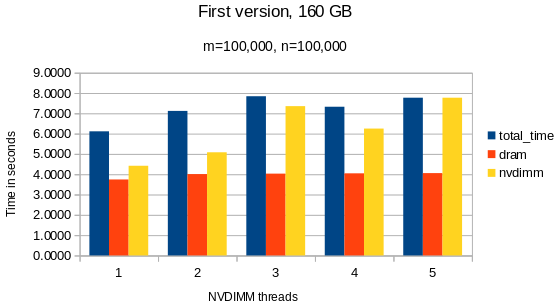
\includegraphics[scale=0.7]{Large_Array_test/First_version_160GB.png}
\caption{Result of the first version of the code with 160 GB of data in graph form.}
\label{fig:FirstVersion160GB}
\end{figure}

\clearpage
\subsection{Second program version}
Same as the first version there are two groups of threads that work in parallel in this program. The first group of threads works on the part of the data that is stored on DRAM and the other works on the data stored on NVDIMM.
In this version the two threads that have a row of elements with neighbors in the other type of memory will not directly access this data. Instead the two arrays will have their own ghost array on their memory that they will access instead of fetching data from the other side. 

The while loop in line 1 will repeat itself for K\_length amount of time usually ten times, this is decided by the user of the benchmark. All the threads will wait for all the other threads to arrive at line 2 before one of the threads will start the time measurement in line 5.
When the threads arrives at line 8 all the DRAM threads will pass the if-test and all the NVDIMM threads will move on to line 19. The DRAM threads will first start the time measurement in line 9 and will then start to calculate the average for every elements in the  part of the array that has been allocated to the each of the threads, this will happen from line 10-17. The threads will then stop the time measurement in line 18.

The NVDIMM threads will enter the else bracket at line 19. The threads will then start time measurement at line 20. From line 21-28 the threads will calculate average on the elements that have been assigned to each thread. At line 29 the threads will stop the time measurements.

The DRAM and NVDIMM threads will then encounter a barrier at line 31 where they will wait for all the other threads to finish. All threads will then update the ghost arrays at line 34 and 35. At line 34 the threads are copying the second row in the NVDIMM array into the last row in the DRAM array. In line 35 they are copying the second last row in the DRAM array into the first row in the NVDIMM array.

Once all the threads are done copying their parts of the rows, one thread will enter the single bracket at line 37. This thread will swap the DRAM arrays and then the NVDIMM array. The thread will then stop the time measurement that was at the beginning of the while-loop at line 47. At line 48 the k variable gets increased by one. The threads will then return to line 1. 

\begin{lstlisting}[caption=Second version of the code where the threads are using ghost array instead of accessing the other type of memory directly.]
while(k<K_length){
	#pragma omp barrier
	#pragma omp single
	{
		total_time[k] = mysecond();
	}
	//Divides threads into DRAM threads and NVDIMM threads.
	if( thread_id < dram_threads ){
		individual_time[k][thread_id] = mysecond();
		for( i=slice_start; i<slice_end; i++){
			for( j=1; j<nMinusOne; j++){
				temp = A[i-1][j-1] + A[i-1][j] + A[i-1][j+1]+
						A[i][j-1]       +       A[i][j+1]+
						A[i+1][j-1] + A[i+1][j] + A[i+1][j+1];
				B[i][j] = temp*inverseEigth;
			}
		}
		individual_time[k][thread_id] = mysecond() - individual_time[k][thread_id];
	}else{
	individual_time[k][thread_id] = mysecond();
		for( i=slice_start; i<slice_end; i++){
        	for( j=1; j<nMinusOne; j++){
        		temp = D_RO(C)[(i-1)*n+(j-1)] + D_RO(C)[(i-1)*n+j] + D_RO(C)[(i-1)*n+(j+1)]+
        				D_RO(C)[i*n+(j-1)]            +            D_RO(C)[i*n+(j+1)]+
        				D_RO(C)[(i+1)*n+(j-1)] + D_RO(C)[(i+1)*n+j] + D_RO(C)[(i+1)*n+(j+1)];
        		D_RW(D)[i*n+j] = temp*inverseEigth;
        	}
        }
		individual_time[k][thread_id] = mysecond() - individual_time[k][thread_id];
	}
	#pragma omp barrier
	#pragma omp for
	for(a=0; a<n; a++){
		A[dram_part_Minus_One][a] = D_RO(C)[n+a];
		D_RW(C)[a] = A[dram_part_Minus_Two][a];
	}
	#pragma omp single
	{
		tempArray = B;
		B=A;
		A=tempArray;

		temp_nvdimm = C;
		C = D;
		D = temp_nvdimm;

		total_time[k] = mysecond() - total_time[k];
		k++;
	}
	#pragma omp barrier
}//End of while
\end{lstlisting}


\begin{table}[!hbtp]
\centering
\begin{tabular}{ |c|c|c|c|c|c|c|c| }
\hline
&  & NVDIMM & DRAM & NVDIMM & DRAM & NVDIMM & Total \\
M & N & rows & threads & threads & time & time & time \\
\hline
31623 & 31623 & 750 & 15 & 1 & 0.2695 & 0.3121 & 0.3138 \\
\hline
31623 & 31623 & 1494 & 14 & 2 & 0.2724 & 0.3115 & 0.3135 \\
\hline
31623 & 31623 & 2315 & 13 & 3 & 0.2730 & 0.3186 & 0.3196 \\
\hline
31623 & 31623 & 3126 & 12 & 4 & 0.2965 & 0.3258 & 0.3367 \\
\hline
31623 & 31623 & 3817 & 11 & 5 & 0.2998 & 0.3196 & 0.3205 \\
\hline
\end{tabular}
\caption{Result of the second version of the code with 16 GB of data.}
\label{tab:SecondVersion16GB}
\end{table}

\begin{figure}[!hbtp]
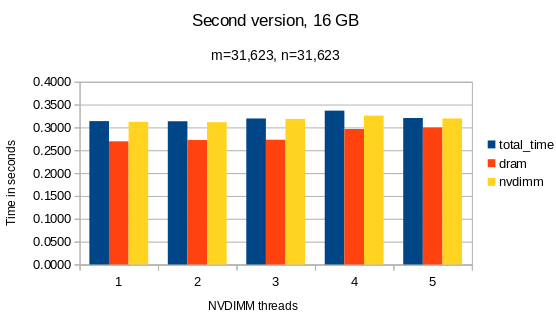
\includegraphics[scale=0.7]{Large_Array_test/Second_version_16GB.png}
\caption{Result of the second version of the code with 16 GB of data in graph form.}
\label{fig:SecondVersion16GB}
\end{figure}

When comparing the predicted DRAM time in table \ref{tab:Prediction16GB} to the measured DRAM time in table \ref{tab:SecondVersion16GB} one can see that at most the prediction is off by between 0.01 and 0.05 seconds.
The prediction DRAM time in table \ref{tab:Prediction160GB} is also quite accurate when compared to DRAM times measured in table \ref{tab:SecondVersion160GB}. The actual result is slower than the predicted time by between 0.2 and 0.5 seconds depending on how many threads have been given to NVIDMM.

The measured time of the NVDIMM in table \ref{tab:SecondVersion16GB} is slower than the predicted time in table \ref{tab:Prediction16GB}. The NVDIMM result is about 0.06 second slower than the predicted result, in percent it is around 20\% slower. 
The NVIDMM result in table \ref{tab:SecondVersion160GB} is also slower than the predicted NVDIMM time in \ref{tab:Prediction160GB}. All the NVDIMM times are between 1 and 2.5 second slower, in percent it would be between 23\% and 37\%.

All the total times in table \ref{tab:SecondVersion16GB} are also almost identical to the NVDIMM time. In this version of the code all threads will update the ghost arrays when all of them are done with the their task so it was expected that the total time was a little slower than the NVDIMM time. The ghost arrays might be so small that they do not have any significant impact on the time.

The total time in table \ref{tab:SecondVersion160GB} is also slower than the NVDIMM time. This is because of the same reasons as mention in last paragraph. The lowest difference between NVDIMM and total time is when just one thread is delegated and the difference is 0.11 seconds. The size of the ghost arrays does not change even though the amount of data on the NVDIMM increases, the length of the ghost arrays is always 100,000 elements. Because of this the difference between total time and NVDIMM should be the same for all the total time. This is not the case, all the other differences are between 0.65 and 1.16 seconds. There is no clear reason for why the test takes that long.

\begin{table}[!hbtp]
\centering
\begin{tabular}{ |c|c|c|c|c|c|c|c| }
\hline
&  & NVDIMM & DRAM & NVDIMM & DRAM & NVDIMM & Total \\
M & N & rows & threads & threads & time & time & time \\
\hline
100000 & 100000 & 2371 & 15 & 1 & 4.1319 & 4.8735 & 4.9889 \\
\hline
100000 & 100000 & 4724 & 14 & 2 & 4.0864 & 5.0859 & 6.0841 \\
\hline
100000 & 100000 & 7321 & 13 & 3 & 4.0079 & 5.5318 & 6.6954 \\
\hline
100000 & 100000 & 9885 & 12 & 4 & 4.1450 & 5.7829 & 6.5336 \\
\hline
100000 & 100000 & 12071 & 11 & 5 & 4.3569 & 6.0666 & 6.7233 \\
\hline
\end{tabular}
\caption{Result of the second version of the code with 160 GB of data.}
\label{tab:SecondVersion160GB}
\end{table}
\begin{figure}[!hbtp]
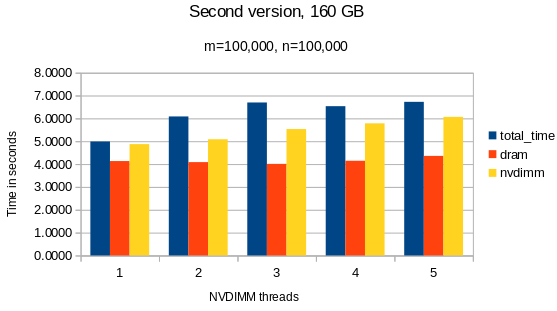
\includegraphics[scale=0.7]{Large_Array_test/Second_version_160GB.png}
\caption{Result of the second version of the code with 160 GB of data in graph form.}
\end{figure}

%\clearpage
\subsubsection{Comparisons of versions}
When comparing the two versions it's possible to make a couple of observations. 
First in the 16 GB test the second version NVDIMM time and total time are faster in all instances and the DRAM in second version is faster three out of five times. The first version of DRAM time is barely faster than the second version of the test two times. 

In the 160 GB version of the test all the total time in the second version are faster then the first version. Three NVDIMM times and one DRAM time in the second version are faster then the first version.

%Since there is no updating of the ghost array in the first version it should be faster then the second version, but this is not the case. In both the 16 GB and the 160 GB version the second version have a faster total time then the first version. If the total time in the first version were equal to NVDIMM which it should theoretically be then first version would have been faster then the second version in two instances. 

Based on the result in the first and second versions, the extra work of updating the ghost array does not make the second version slower then the first version. The code in the second version is also more readable than the first version because it does not have all of the if-sentences and code that repeats itself. 

Overall the second version is the better version based on the total time and the readability of the code. 


\clearpage
\section{DRAM and NVDIMM working independently}
\label{Chapter:workingIndepandently}
\subsection{Introduction}
In the tests that was done in chapters three and four the DRAM and NVDIMM have been doing the same type of work. This chapter will be about DRAM and NVDIMM doing different types of work. 
There will be a group of threads calculating data on DRAM. While this is going on there will be another group of threads copying the latest set of calculated data to NVDIMM and analyzing the data on NVDIMM.
The purpose of this is to find out if NVDIMM can work on other tasks and understand how NVDIMM is behaving when other threads are working on DRAM.
The chapter will start by testing the DRAM alone in order to see what kind of performance is possible. Afterward another version of the program will be tested where both DRAM and NVDIMM are being used. 

\subsection{Test with only DRAM}
\label{section:DramOnly}
\subsubsection{Description of code}
The code in \ref{lst:DramOnlyMain} starts by taking a time measurement before the while-loop in line 4 by on of the threads. This time measurement will be ended after the while-loop at line 41 by one thread. Since there is a barrier at line 38 the time measurement will only end when all the threads have left the while-loop.

The While-loop at line 6 will be repeated for 5000 times and there is a barrier in line 7 to ensure that all threads are finished with the previous iteration before starting a new iteration. One thread will start by entering a single bracket in line 8 and does all the work only one thread can do such as increase n by one, zero out diff and average and does a calculation in line 13 that result will be used by all the threads later.
%a part of a formula that will be used in data generation.
The description of data generation will be done in section \ref{sec:dramOnlyDatagen}.

After the data generation all the threads will wait the barrier at line 19 before one thread enters the single bracket at line 20. The thread will swap the arrays x and xk\_1 before starting a new time measurement at line 26.
The threads will move on to analyzing the data generated and this will be described at section \ref{sec:dramOnlyAnalyze}.

The threads will wait for all the threads to complete analyzing the data at line 31 before on thread enter a new single at line 32 where it will first start by calculating an average and after that it will end the time measurement that was started at line 26. This is the time measurement of the analyzing part of the code, the time it takes to analyze the data in all iterations will be add to one variable called analyze\_time. This is the end of the while-loop and the code will either return to line 7 or exit the while-loop

The time measurement of the data generation will be found by subtracting analyze\_time from the time measurement that was taken before and after the code. 

%[caption=while-loop]
\begin{lstlisting}[caption={DRAM only version of the simulation code.},escapeinside={{/*!}{!*/}}, label={lst:DramOnlyMain}]
double double_temp;
#pragma omp single
{
	data_generation_time, = mysecond();
}
while( n<5000 ){
	#pragma omp barrier
	#pragma omp single
	{
		n++;
		diff=0.0;
		average = 0;
		//completes the first part of the formula.
		Wk_1_product = (omd + (d*Wk_1))*iN;
	}
	
	Data generation, see section /*!\ref{sec:dramOnlyDatagen}!*/
	
	#pragma omp barrier
	#pragma omp single
	{
		temp_x = xk_1;
		xk_1 = x;
		x = temp_x;
		//starting time measurement of calculation.
		temp_calc=mysecond();
	}
	
	Analyzing the data, see section /*!\ref{sec:dramOnlyAnalyze}!*/
	
	#pragma omp barrier
	#pragma omp single
	{
		average *= iN;
		analyze_time+=mysecond()-temp_calc;
	}
}
#pragma omp barrier
#pragma omp single
{
	data_generation_time, = mysecond() - data_generation_time;
}
\end{lstlisting}
The code shown in listing \ref{lst:DramOnlyTimeMeasurement} is the function used to take the time measurement. This function has been copied from the Stream benchmark code. 
\begin{lstlisting}[caption={Function that that is used for measure time},escapeinside={{/*!}{!*/}}, label={lst:DramOnlyTimeMeasurement}]
double mysecond(){
	struct timeval tp;
	struct timezone tzp;
	int i;
	i = gettimeofday(&tp,&tzp);
	return ( (double) tp.tv_sec + (double) tp.tv_usec * 1.e-6 );
}
\end{lstlisting}
%\clearpage
\subsubsection{Data generation}
\label{sec:dramOnlyDatagen}
All the threads will enter the for-loop at line 2 and they will start by zero out the double\_temp variable. They will then enter a new for-loop at line 5.
The array used in this test is a compressed row storage(CRS), this means that a 2D-array has been converted to an 1D-array where all the elements with zero have been removed. CRS\_row\_ptr shows the where a row in the 2D-array begins and ends in the CRS, that is why the CRS\_row\_ptr is used in the header of the for-loop. At line 6 the for-loop will multiply together all elements in a row together with the result from a previous iteration of data generation. 
Everything will be added together in the variable double\_temp. The variable double\_temp will then be multiplied with a constant d at line 9 and added together with a constant Wk\_1\_product at line 11 before being stored in array x at line 12 which is where data from the current data generation is being stored.
The code will then check if the difference between current data generation and previous data generation is higher than the diff variable. If it is then the diff variable will be changed to the current difference.

\begin{lstlisting}[caption=Generation of data.]
#pragma omp for reduction(max:diff)
for( i=0; i<nodes; i++){
	//This is A*x^k-1
	double_temp = 0;
	for( j=CRS_row_ptr[i]; j<CRS_row_ptr[i+1]; j++){
		double_temp += CRS_values[j] * xk_1[CRS_col_idx[j]];
	}
	//d*Ax^k-1
	double_temp *= d;
	//Adding the first part and second part together.
	double_temp += Wk_1_product;
	x[i] = double_temp;

	//Comuting the difference between x^k and x^k-1
	//and adds the biggest diff to diffX[thread_id]
	if( x[i]-xk_1[i] > diff ){
		diff = x[i] - xk_1[i];
	}
}
\end{lstlisting}


\clearpage
\subsubsection{Analyzing the data}
\label{sec:dramOnlyAnalyze}
%The analyzing part of the code runs through the nodes array 
This analysis code is very synthetic and therefore it will go through the array five times and add all the elements to the variable called average, this is shown in the code in listing \ref{lst:DramOnlyAnalyzing}. The average is calculated five times in a row in order to make the analysis part heavier.

\begin{lstlisting}[caption={Analyzing the data.},escapeinside={{/*!}{!*/}}, label={lst:DramOnlyAnalyzing}]
//Analyse part
#pragma omp for reduction(+ : average)
for(i=0;i<nodes;i++){
	average += xk_1[i];
}
#pragma omp for reduction(+ : average)
for(i=0;i<nodes;i++){
	average += xk_1[i];
}
#pragma omp for reduction(+ : average)
for(i=0;i<nodes;i++){
	average += xk_1[i];
}
#pragma omp for reduction(+ : average)
for(i=0;i<nodes;i++){
	average += xk_1[i];
}
#pragma omp for reduction(+ : average)
for(i=0;i<nodes;i++){
	average += xk_1[i];
}
\end{lstlisting}

\subsubsection{Result}
\begin{table}[!hbtp]
\centering
\begin{tabular}{ |c|c|c|c| } 
\hline
Threads &  Total time & Data generation time &  analysis time \\
\hline
1 & 1545.98 & 949.60 & 596.38 \\
\hline
2 & 671.34 & 421.51 & 249.82 \\
\hline
3 & 459.76 & 289.57 & 170.18 \\
\hline
4 & 350.04 & 220.99 & 129.05 \\
\hline
5 & 284.09 & 179.43 & 104.66 \\
\hline
6 & 240.27 & 151.90 & 88.37 \\
\hline
7 & 209.05 & 132.54 & 76.51 \\
\hline
8 & 188.60 & 120.08 & 68.52 \\
\hline
9 & 177.25 & 113.20 & 64.05 \\
\hline
10 & 168.02 & 109.87 & 58.15 \\
\hline
11 & 159.60 & 106.06 & 53.54 \\
\hline
12 & 152.81 & 103.37 & 49.44 \\
\hline
13 & 150.41 & 101.86 & 48.55 \\
\hline
14 & 146.30 & 100.99 & 45.31 \\
\hline
15 & 143.02 & 100.55 & 42.47 \\
\hline
16 & 140.75 & 100.74 & 40.01 \\
\hline
\end{tabular}
\caption{Result from running the test with only DRAM. The time is measured in seconds.}
\label{tab:DramOnlyResult}
\end{table}

The result of the test with only DRAM is shown in table \ref{tab:DramOnlyResult}. This result will be compared to result where DRAM is working data generation and NVDIMM is transferring the result of data generation to NVDIMM and analyzing the result there.

%\clearpage
\pagebreak
\subsection{NVM simulation}
\subsubsection{Locks}
The program is divided into two parts, the calculation of data and the analyzing of the data that have been generated. The two parts synchronize by using two locks called lock\_a and lock\_b, lock\_a will start in unlocked state and lock\_b in locked state. When the two parts start the analyzing part is put on hold by lock\_b until the calculation part has generated the first set of data. Then the calculation part will lock lock\_a, swap the pointers x and xk\_1 and then unlock lock\_b. The calculation part will then start the calculation of the next set of data, but wont swap pointers until analyzing part has transferred the content in xk\_1 to NVDIMM and unlocked lock\_a.

When the calculation part unlocks lock\_b the analyzing will start transferring data from xk\_1 to NVDIMM and unlock lock\_a when it's done with the transfer. The analyzing part will then start analyzing the data on NVDIMM. When it's done it will encounter lock\_b and will wait there until calculation has a new set of data ready and has swapped the pointers.

Before and after the set lock in calculation and analyze part there is a time measurement that measured how long the threads have waited for the lock to be unlocked by the other part. All the individual times the threads have waited in calculation or analyze gets added to a variable called iteration\_idle\_time or transfer\_idle\_time that will be the total time the threads have waited. 

%lock_overview.png
\begin{figure}[!hbtp]
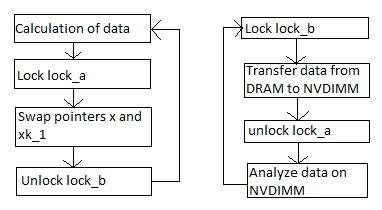
\includegraphics[scale=1]{lock_overview.png}
\caption{A simplified version of how lock works in the program.}
\end{figure}

\subsubsection{Calculation}
The total time for calculation is measured before and after the while-loop. One thread will start the time measurement at line 3 and the measurement will be ended by one thread at line 33.
The calculation starts with a while-loop at line 5. It will be repeated 5000 times. There is a barrier at line 6 that will synchronize all the threads. One thread will enter a single bracket a line 7 and increase the variable n by one, zero out the variables diff and Wk\_1 and calculate one part of the calculation that only need to be done by one thread at line 11.

The calculation of data will happen at line 17. All threads will enter the for-loop at line 18, this for-loop will pass through all the nodes in the array. A temporary variable is created at line 20, this is to ensure that data is only stored at the end of the for-loop. Each thread will then enter a second for-loop at line 21. The array that begins with CRS is part of a compressed sparse matrix, that means that a 2D-array has been turned into a 1D-array in order to perform faster. The for-loop will add together edges that are connected to node i, they will be stored in the double\_temp variable. Once out of the array the double\_temp will be multiplied with a constant d at line 25 and added together with the Wk\_product at line 27, this is a variable that was calculated by one thread in line 13.
The double\_temp value will be written to array at line 28.

One thead will enter the single bracket at line 36 and will start a new time measurement at line 38. This time measurement will measure how much time the calculation threads must wait for the analyze threads to finish. Once the analyze threads have unlocked lock\_a the thread will pass through the lock and lock it again at line 39. It will also end the time measurement at line 40 and add the time waited to the iteration\_idle\_time variable. This variable is the total amount of time the calculation threads have been idle.
At line 42-44 the arrays x and xk\_1 will be swapped. At line 46 the thread will unlock the lock\_b, this will allow the analyze threads to do their jobs. The threads will then return to the beginning of the while-loop at line 5 and repeat the process if n is lower than 5000.


\begin{lstlisting}[caption=Calculation]
#pragma omp single
{
	iteration_time = mysecond();
}
while( n<5000 ){ 
	#pragma omp barrier
	#pragma omp single
	{
		n++;
		diff=0.0;	
		Wk_1=0;
		//completes the first part of the formula.
		Wk_1_product = (omd + (d*Wk_1))*iN;
	}
	
	/* Calculation of Data */
	#pragma omp for reduction(max:diff)
	for( i=0; i<nodes; i++){
		//This is A*x^k-1
		double_temp = 0;
		for( j=CRS_row_ptr[i]; j<CRS_row_ptr[i+1]; j++){ 
			double_temp += CRS_values[j] * xk_1[CRS_col_idx[j]];
		}
		//d*Ax^k-1
		double_temp *= d;
		//Adding the first part and second part together.
		double_temp += Wk_1_product;
		x[i] = double_temp;

		//Comuting the difference between x^k and x^k-1
		//and adds the biggest diff to diffX[thread_id]
		if( x[i]-xk_1[i] > diff )
			diff = x[i] - xk_1[i];
	}

	#pragma omp single
	{
		temp_time = mysecond();
		omp_set_lock(&lock_a);
		iteration_idle_time += mysecond() - temp_time;

		temp_x = xk_1;
		xk_1 = x;
		x = temp_x;
		
		omp_unset_lock(&lock_b);
	}
}//end of while-loop
#pragma omp single
{
	iteration_time = mysecond() - iteration_time;
}
\end{lstlisting}
\subsubsection{Analysis}
The time will be measured before and after the while-loop that start at line 1. The if test for this while-loop has been moved to the end of the while-loop, that is why the if test at line 1 is 1==1 and will allways be true. 
One thread will enter the single bracket at line 2 and start a time measurement that will measure the idle time of the analyze threads. The threads will wait until the calculation threads unlock the lock\_b. When it's unlocked the thread will pass through line 5 and lock lock\_b again. It will also add the time waited to the variable transfer\_idle\_time. The thread will then start a new time measurement at line 7, this measurement will measure the time it takes to transfer data from DRAM to NVDIMM. the variable average will be turned to zero at line 8.
At line 11-14 all the threads will work together to transfer the xk\_1 array from DRAM to NVDIMM.
Once done one thread will enter a new single at line 15. The thread will then end the time measurement at line 17 and add the time taken to transfer the data to the variable DRAM\_to\_NVM\_time.
It will then unlock lock\_a at line 18, this will allow the calculation threads to swap x and xk\_1. The thread will also start a new time measurement at line 19, this measurement will measure how long it takes for the threads to analyze the data. Line 22-25 is where the data gets analyzed, in this case it's just an average of all the data. 
The threads will synchronize at a barrier at line 26. One thread will enter the single thread at line 27 and will divide the sum of all the nodes with the number of nodes.
It will then end the time measurement at line 30 and add it to the total time it takes to analyze the data.
All the threads will then go through an if test at line 33. This test will always be true until the calculation threads changes the iteration\_ongoing variable from 1 to 0.This will only be done when calculation threads are done with calculation and left their while-loop that was explained above.

\begin{lstlisting}[caption=Analyze]
while(1==1){
	#pragma omp single
	{
		temp_time = mysecond();
		omp_set_lock(&lock_b);
		transfer_idle_time += mysecond() - temp_time;
		temp_time = mysecond();
		average=0.0;
	}
	/* Transfer of array from DRAM to NVDIMM */
	#pragma omp for
	for(i=0; i<nodes; i++){ 
		D_RW(nvm_values)[i]=xk_1[i];
	}
	#pragma omp single 
	{
		DRAM_to_NVM_time += mysecond() - temp_time;
		omp_unset_lock(&lock_a);
		temp_time = mysecond();
	}
	/* Analyzations of data */
	#pragma omp for reduction(+ : average)
	for(i=0;i<nodes;i++){
		average += D_RO(nvm_values)[i];
	}
	#pragma omp barrier
	#pragma omp single
	{
		average /= nodes;
		Analyse_time += mysecond() - temp_time;
	}
	//if sentence for exiting while-loop.
	if(iteration_ongoing==0){
		break;
	}
}
\end{lstlisting}

\pagebreak
\subsubsection{Prediction}
%Table \ref{tab:nvmPredictions} shows the time prediction that the code above will take. Column one and two shows the number of DRAM and NVDIMM threads that are being used. The last three columns shows the predicted times for data generation on DRAM, transfer of data from DRAM to NVDIMM and the analyzing of data in NVDIMM. The speeds used to predict times comes from benchmarks in section \ref{section:NVM-NVM} and \ref{section:DRAM-NVM}. The calculation of the data traffic data generation and analyzing of data in this prediction is the same as the one in figure \ref{fig:DramOnlyMath1} and \ref{fig:DramOnlyMath2}. The data traffic for the data transfer from DRAM to NVDIMM is calculated in figure \ref{fig:DramOnlyMath3}.
Table \ref{tab:nvmPredictions} shows the prediction of how much time it will take to transfer data from DRAM to NVDIMM. First and second columns show the number of DRAM and NVDIMM threads. Third column shows the transfer speed in MB/s. These speed has been taken from benchmark in section \ref{section:DRAM-NVM}. The fourh column shows the total amount of time it took to transfer data from DRAM to NVIDMM.

The equation below show the calculation of how much data would be transferred from DRAM to NVDIMM. Nodes is the number of elements in the array that will be transferred 5000 times from DRAM to NVDIMM. That result is multiplied with 8 and divided by 1,000,000 in order to convert  the result to megabyte.

\begin{equation}
	Data = \frac{nodes*5000*8}{1000000}
\end{equation}
%\caption{Calculation of data traffic generated by transferring data from DRAM to NVDIMM, result is measured in megabytes.}
%\label{fig:DramOnlyMath3}
\begin{table}[!hbtp]
\centering
\begin{tabular}{ |c|c|c|c| } 
\hline
DRAM & NVM & DRAM-NVDIMM & transfer \\
theads & threads & speed in MB/s & time \\
\hline
15 & 1 & 3581.48 & 178.70 \\
\hline
14 & 2 & 7323.96 & 87.38 \\
\hline
13 & 3 & 10954.06 & 58.43 \\
\hline
12 & 4 & 15070.61 & 42.47 \\
\hline
11 & 5 & 18725.90 & 34.18 \\
\hline
10 & 6 & 22614.45 & 28.30 \\
\hline
9 & 7 & 26557.71 & 24.10 \\
\hline
8 & 8 & 30570.88 & 20.93 \\
\hline
7 & 9 & 33996.95 & 18.83 \\
\hline
6 & 10 & 38191.10 & 16.76 \\
\hline
5 & 11 & 42263.28 & 15.14 \\
\hline
4 & 12 & 45915.39 & 13.94 \\
\hline
3 & 13 & 49341.90 & 12.97 \\
\hline
2 & 14 & 53331.10 & 12.00 \\
\hline
1 & 15 & 57348.14 & 11.16 \\
\hline
\end{tabular}
\caption{Time prediction in seconds of the data transfer between DRAM and NVDIMM.}
\label{tab:nvmPredictions}
\end{table}

\pagebreak
\subsubsection{Result}
\begin{enumerate}[A.]
\item Threads used for data generation.
\item Threads used for transferring data from DRAM to NVDIMM and analyzing the data.
\item Data generation time.
\item Idle time for threads allocated to data generation.
\item Transfer time for data between DRAM and NVDIMM.
\item Analysis time
\item Idle time for threads allocated to transfer data and analysis.
\item Total time used.
\end{enumerate}

\begin{table}[!hbtp]
\centering
\begin{tabular}{ |c|c|c|c|c|c|c|c| } 
\hline
A & B & C & D & E & F & G & H \\
\hline
15 & 1 & 102.35 & 849.87 & 166.02 & 786.30 & 0.03 & 952.37 \\
\hline
14 & 2 & 105.89 & 402.37 & 84.74 & 423.54 & 0.04 & 508.35 \\
\hline
13 & 3 & 112.69 & 274.05 & 70.52 & 316.22 & 0.03 & 386.80 \\
\hline
12 & 4 & 117.66 & 181.92 & 51.48 & 248.09 & 0.01 & 299.63 \\
\hline
11 & 5 & 123.18 & 126.36 & 43.15 & 206.36 & 0.03 & 249.58 \\
\hline
10 & 6 & 130.29 & 90.92 & 44.56 & 176.63 & 0.03 & 221.25 \\
\hline
9 & 7 & 136.33 & 51.77 & 34.79 & 153.22 & 0.10 & 188.13 \\
\hline
8 & 8 & 147.03 & 18.63 & 31.22 & 134.42 & 0.03 & 165.69 \\
\hline
7 & 9 & 169.39 & 3.78 & 36.38 & 120.80 & 16.01 & 173.20 \\
\hline
6 & 10 & 182.96 & 0.02 & 28.85 & 102.81 & 51.34 & 183.01 \\
\hline
5 & 11 & 206.64 & 0.00 & 26.39 & 90.11 & 90.16 & 206.67 \\
\hline
4 & 12 & 246.10 & 0.31 & 28.67 & 90.41 & 127.23 & 246.46 \\
\hline
3 & 13 & 303.90 & 0.00 & 22.83 & 75.71 & 205.38 & 303.93 \\
\hline
2 & 14 & 430.30 & 0.00 & 21.71 & 69.86 & 338.74 & 430.34 \\
\hline
1 & 15 & 804.03 & 0.00 & 20.60 & 65.07 & 718.38 & 804.08 \\
\hline
\end{tabular}
\caption{Result where DRAM and NVDIMM does different tasks, all times measured in seconds. Symbols in top row are explained above the table.}
\label{tab:NVMresults}
\end{table}

The prediction of the data transfer was correct for the most part. The predictions with one and two NVDIMM threads were above the measured time in table \ref{tab:NVMresults}. All the other predictions are lower than the measured time. Since almost all the prediction are lower than the measured time it could be used as prediction of minimum time needed for transferring data from DRAM to NVDIMM.

%The prediction of data generation and the analyze time in table \ref{tab:nvmPredictions} is always slower than the measured result in table \ref{tab:nvmDataGenerationTimes}. They could serve as a prediction of maximum time needed for the data generation and analyzing of data to complete their tasks. The prediction of the data transfer is less reliable then the others. This is because it predict more time then what the actual time is in the beginning and at the end it predict less time then what is actually needed. It cant be used to predict a maximum time or a minimum time needed for the transfer of data between DRAM and NVDIMM.

The fastest combination of DRAM and NVDIMM thread in this test is when both DRAM and NVDIMM have eight threads. This is also the combination where the combined idle time of the two groups of threads are the lowest which is also the reason why it was the fastest one. 

The fastest combination result in this section is 25 second slower when compared to the fastest result of DRAM only version of the code in table \ref{tab:DramOnlyResult}. It was expected that the NVDIMM version of the code would be slower than the DRAM only version of the code. But still it is possible to assign the DRAM with one set of tasks while the NVDIMM version of the code is doing another set of tasks. The only downside is that it will take longer time. When comparing the extra time a project will take with the amount of extra space the user gets by using NVDIMM it would probably be worth it. 

\clearpage
\section{Conclusion}
\label{chapter:conclusion}
The conclusion will start with a summary of what has happened in the previous chapters. Then it will move on to answer the research questions that were introduced in the beginning of the thesis. After the research questions have been answered there will be a section with reflections of what could have been done better or differently. The thesis will end with a section that considers what further work could be. 

\subsection{Summary}
This thesis started in chapter \ref{Chapter:Introduction} with explaining what persistent memory is, what are the advantages and disadvantages. Four research questions were introduced in the end of the section that will be answered later in this chapter. 

The thesis continued with explaining the basic when programming with NVDIMM in chapter \ref{Chapter:Basicprogramming}. 

In chapter \ref{Chapter:Benchmarks} I created a modified version of the Stream benchmark that could be used to measure the speed of the NVDIMM. I also created three other benchmark that are similar to each other where the threads are competing with each other for bandwidth. I used the benchmarks to measure the performance of NVDIMM on the computer I used through the entire thesis it is described in section \ref{sec:hardware} and made observation based on those performance measurements. 

Chapter \ref{Chapter:Cooperation} is about DRAM and NVIDMM working together because the amount of data exceeds the total capacity of the DRAM.
I created a formula that calculated how much should be allocated from DRAM to NVDIMM. I also created two versions of a new test that could test if the formula is correct. The purpose of the two versions was to which programming decision is the fastest.

Chapter \ref{Chapter:workingIndepandently} is about NVDIMM and DRAM doing two different types of jobs. I created a new test where DRAM is working on generating data while the NVDIMM is transferring the last set of generated data to from DRAM to NVDIMM and analyzing the data afterward.

\pagebreak
\subsection{Research questions}
\subsubsection{Question 1}
What is the data transfer speed of NVDIMM compared to DRAM?

The expectation before starting this thesis was that NVDIMM would be slower than DRAM. What I focused on is how fast the speed of the NVDIMM is compared to DRAM. This question is possible to answer by comparing the results Stream  benchmark int section \ref{section:STREAMDRAM} and the result from modified Stream benchmark in section \ref{section:STREAM_NVDIMM}. By comparing the speed from these two benchmarks which has been done in table \ref{tab:Q1} in section \ref{section:Observations} it possible to see how much faster the DRAM is.

\subsubsection{Question 2}
In an competitive environment, in what way will NVDIMM and DRAM affect each other?

When both DRAM and NVDIMM are competing for bandwidth the speed will be slower than what they would be if they were alone with the bandwidth. When using all cores in a socket the sum of the DRAM speed and NVDIMM speed will be lower then the speed of sixteen DRAM threads running alone, this can be determined by comparing table \ref{tab:DRAM_STREAM_100M_Table} and \ref{tab:NVM_NVM}.

\subsubsection{Question 3}
When the size of the data is higher than the capacity of the DRAM, how much data should be transferred to NVDIMM? How many threads should be allocated to work on the data on NVDIMM?

In chapter four I created a formula that can be used to find out how much data should be placed on NVDIMM based on what the speed of DRAM and NVDIMM is. By deciding first on how many threads should be allocated the formula will tell how much data should be placed on NVDIMM.

\subsubsection{Question 4}
While DRAM is working on a task, is it possible for NVDIMM to be working on a different type of task?
In chapter \ref{Chapter:workingIndepandently} I created a program where a group of DRAM threads working on one task while a group of NVDIMM threads transfer the the result of that work to NVDIMM and do another type of task on that data. The program is slower than the DRAM version of the program, but it is possible to have DRAM and NVDIMM do different kinds of tasks simultaneously.


\subsection{Reflections}
The benchmark section \ref{section:NVM-NVM}, \ref{section:NVM-DRAM}, \ref{section:DRAM-NVM} had unstable NVDIMM theads that dropped their speed for some reason. More time could have been spent trying to find out why this is occurring.

A part of chapter \ref{Chapter:workingIndepandently} was to predict the time it takes to complete the data generation and analysis part. This was dropped because I were unable to predict it correctly.

While working on this thesis I could have saved a lot of time by having a greater attention to details. By looking at the results more critically I could have noticed mistakes more easier and it would not be necessary for my supervisor to point it out. 

I should also have been more creative in my approach. That would have enabled me to attack a problem from different angles and this thesis might had gotten a different result because of that.

\subsection{Further work}
Further work would be to find out what causes the NVDIMM threads to drop their speed sometimes that was shown in competing benchmark section in chapter three.
If it's possible to explain what causes this it might be possible to make programming choices that avoid the sudden drop from happening. The result is that with no drop in speed it might be possible to get more performance out of NVDIMM.

\clearpage
\printbibliography

\end{document}
